\documentclass[cn,pad,chinesefont=nofont,twocol]{elegantbook}
\usepackage{array}
\usepackage{xpinyin}
\usepackage{latexgit}
\usepackage{hyperref}
\hypersetup{
	pdftitle={北園清箫習谱},
    pdfauthor={北园主人}
}
\setCJKmainfont{Source Han Serif} 
\setCJKsansfont{Source Han Sans} 
\setCJKmonofont{Source Han Mono}

\title{北園習箫谱 - 筒音5}
\author{青箫散人}
\date{\zhtoday}
\cover{cover21}
\logo{monk.png}
\extrainfo{清籁远\xpinyin*{喑}喑,秦楼夜思深。碧空人已去,沧海凤难寻。\\杳妙和云绝,依微向水沉。还将九成意,高阁伫芳音。}
\version{\gitcommithash}
\fancyfoot[C]{明月如霜,青箫独吟,小桥清溪枯柳。杯黄酒,又见纤纤酥手舞彩袖。}

\begin{document}
\maketitle
\frontmatter
\tableofcontents
\mainmatter

\chapter{箫的来历}
\paragraph*{箫,形声。字从竹从肃,肃亦声。“肃”本义为“千针万孔”,转义为“风声尖锐地漫天呼啸”。“竹”与“肃”联合起来表示“一种模拟风声漫天尖锐呼啸的竹制吹奏乐器”。本义:一种模拟风吹声的竹乐器。}
\paragraph*{箫源于远古时期的骨哨,新石器时代开始以竹制作。历史上亦称为笛,在秦汉至唐,箫是指编管的排箫。唐以后方专指竖吹之笛。“横吹笛子竖吹箫”,即笛箫之间最基本的差别。箫历史悠久,音色圆润轻柔,幽静典雅,适于独奏和重奏。} 
\paragraph*{早在《尚书·益稷》中记载有“\xpinyin*{箫韶九成,凤凰来仪}。”当因韶乐伴奏乐器以箫(当时为排箫)为主而有此称。箫在汉代时称为“\xpinyin*{篴}”、“竖篴”。西晋乐工列和、中书监荀勖所改革的笛为6 孔(前5、后1),其形制与今天的箫已非常相似了。东晋的桓伊,擅长音乐,他有一支蔡邕的柯亭笛(箫),是江南数第一的吹箫名手,地位和声望都已很高。他曾为素不相识的王徽之吹奏过三段乐曲,在历史上被传为佳话。}
\paragraph*{魏晋南北朝时,箫已用于独奏、合奏,并在伴奏相和歌的乐队中使用。清代,箫的形制完全一样。清《律吕正义后编》记载:“明时乃直曰箫,不复有竖篴。今箫长一尺八寸弱,从上口吹,有后出孔;笛横吹,无后出孔。”}
\paragraph*{当代箫有三种,分别是琴箫,洞箫和南箫。三种箫最大的区别是管径,音色稍有差异。琴箫最为细腻,南箫在稍显粗狂豪放,洞箫介于二者之间,玩转悠然。日本的尺八,是由唐尺八传到日本。后经过多年改革,并结合日本本土文化形成的日本民族乐器,音色沧桑悲凉。实际上,他们的音色差别并不大,主要是乐曲本身的特色带来的感觉。}

\paragraph*{\textbf{管径参考(mm):}\\
\begin{tabular}[t]{|c|l|l|}
  	\firsthline
           & F调           & G调 \\ \hline
    洞箫    & 外26/内18.5   & 外25/内17-18 \\
    琴箫    & 外24/内15-16  & 外23/内14-15 \\
	\lasthline 
\end{tabular}
}

\begin{center}
	\vfill
	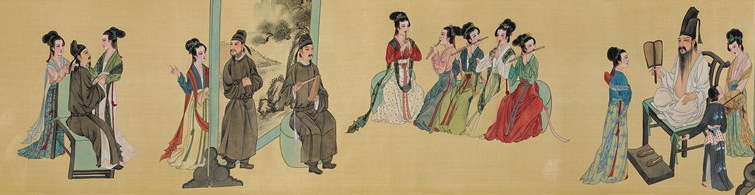
\includegraphics[width=\textwidth]{cover8}
\end{center}

\chapter{指法图}
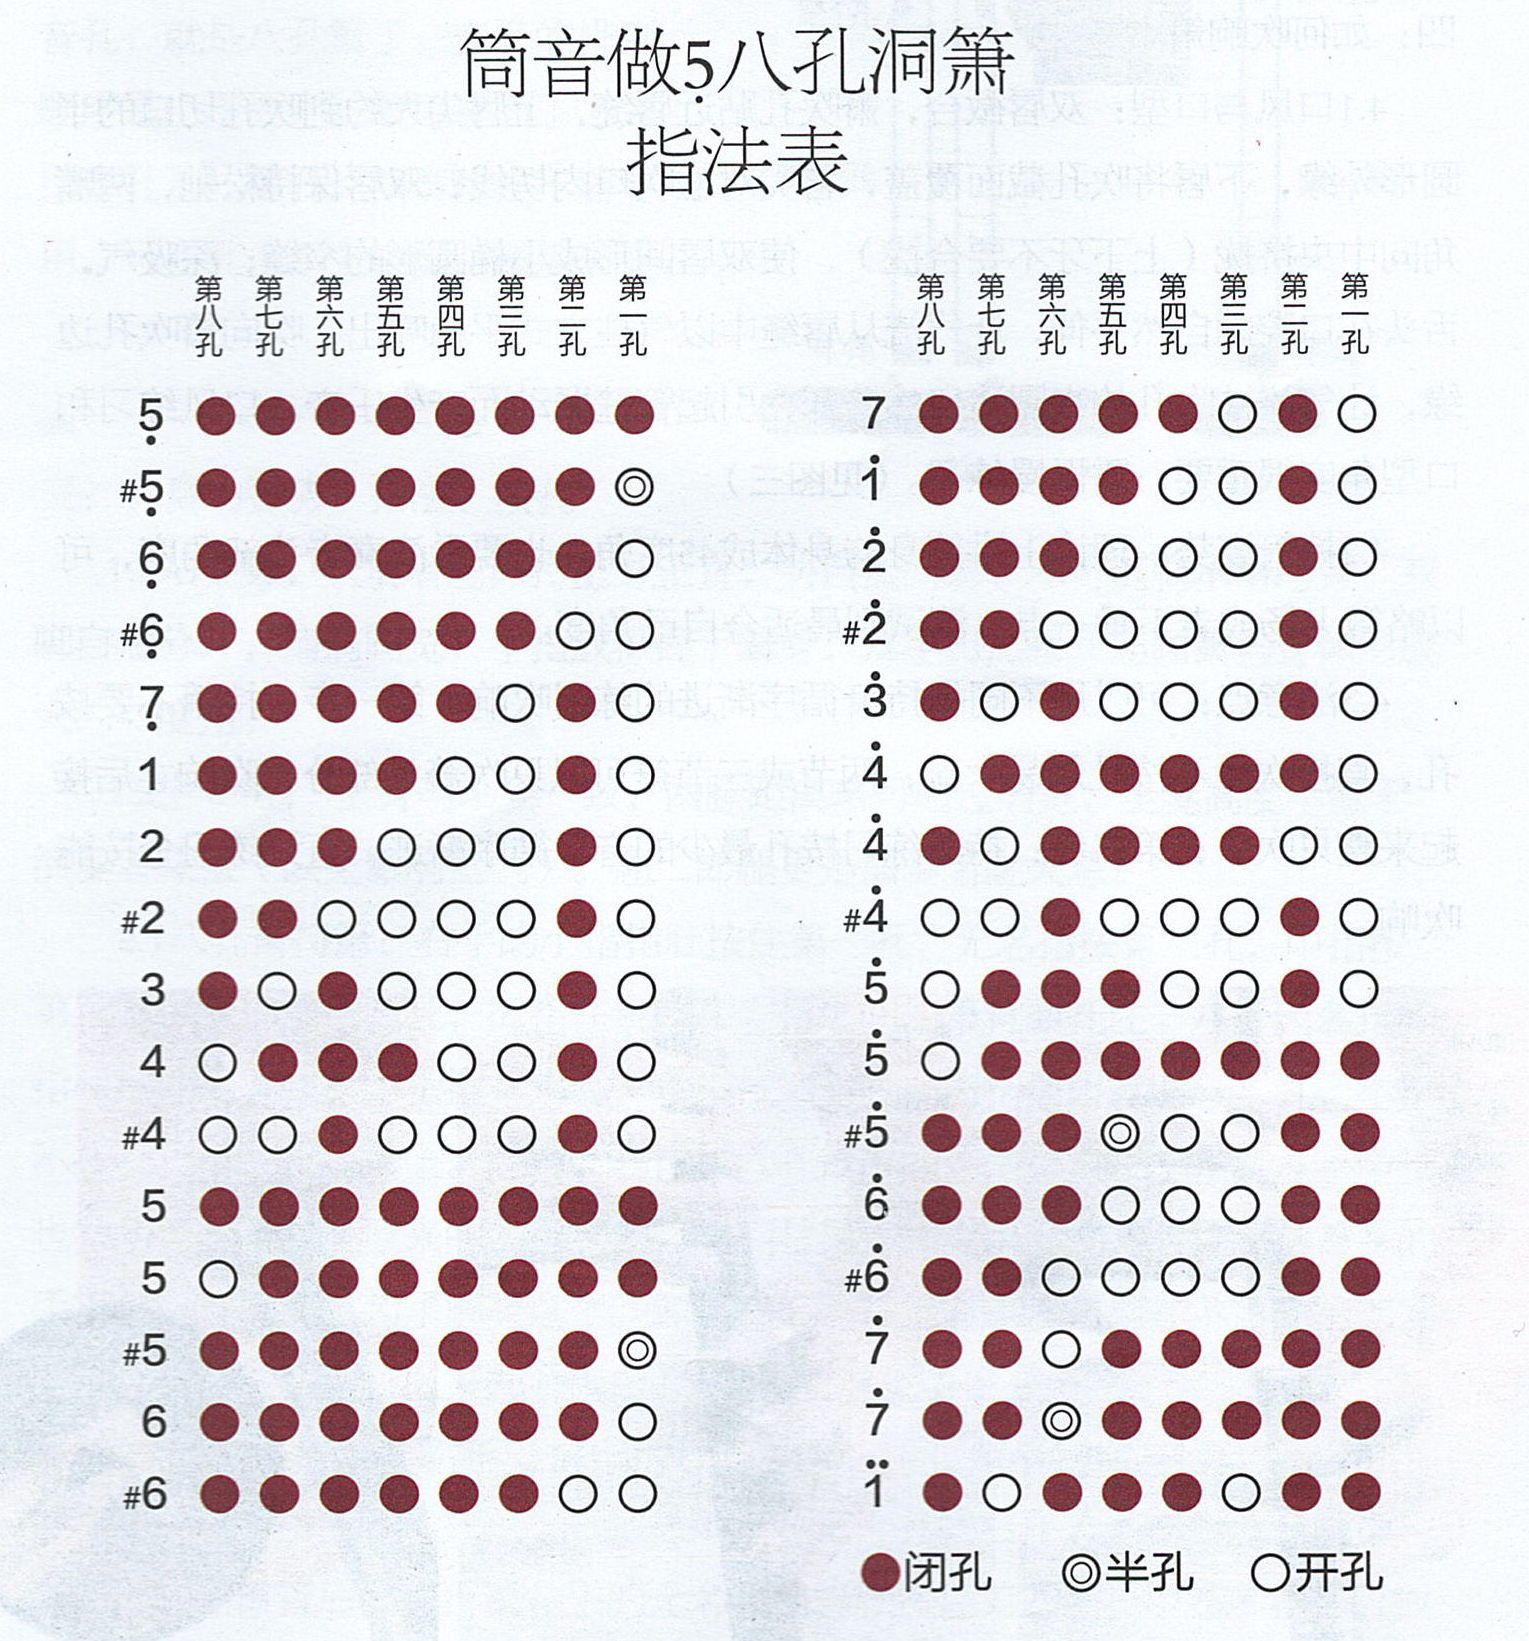
\includegraphics[width=\textwidth]{dongxiao/Scan.jpeg}
\section{补-8孔箫指法(横)} \center
    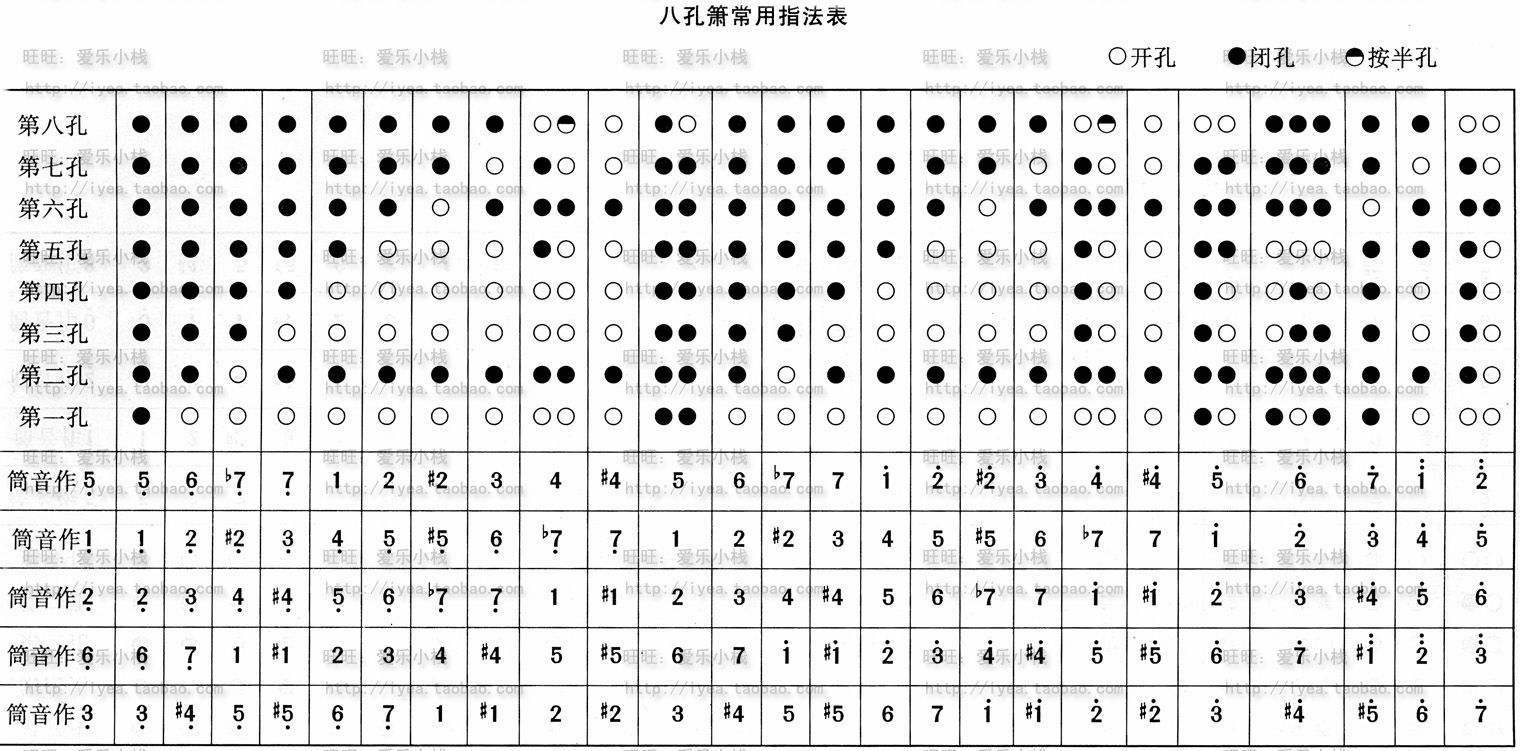
\includegraphics[width=0.94\textheight, angle=90]{dongxiao/20200817-8孔箫指法-横}
\section{补-8孔箫指法(竖)}
    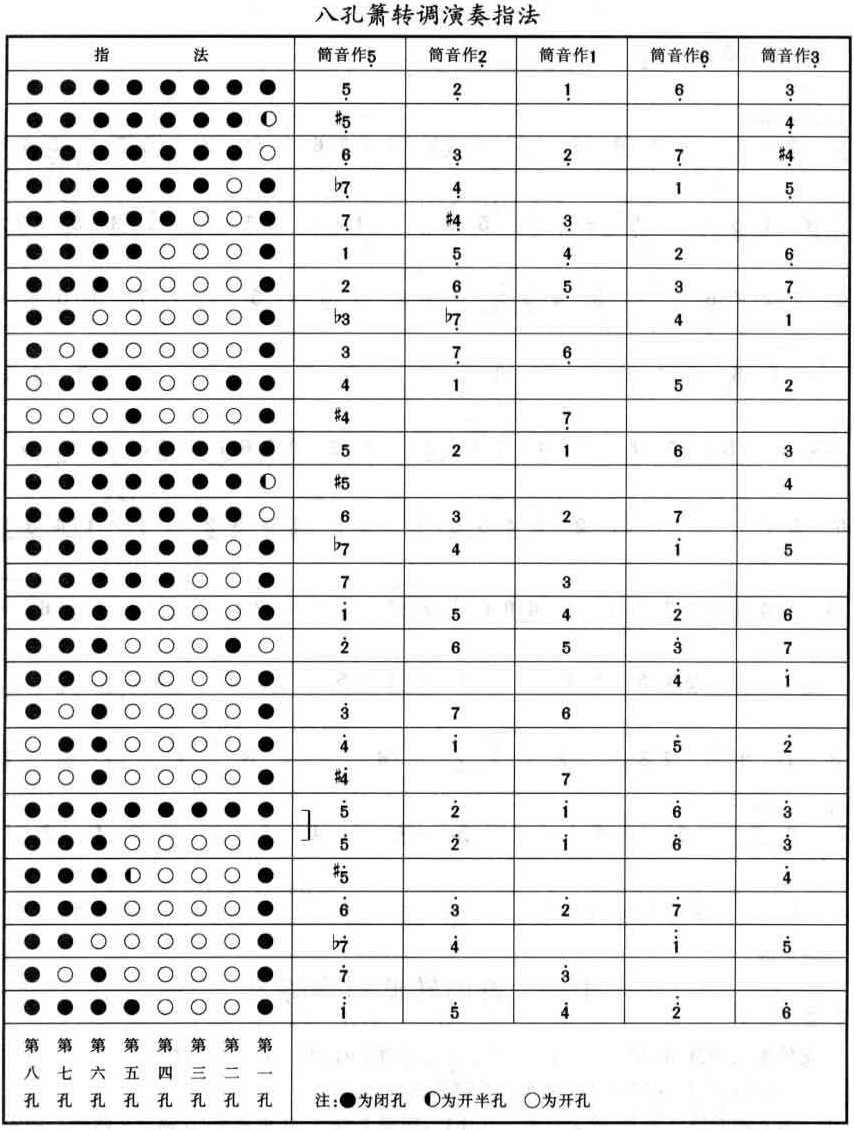
\includegraphics[width=0.9\textwidth]{dongxiao/20200817-8孔箫指法-竖}

\chapter{基礎谱}
\section{筒音作5}
\begin{center}
	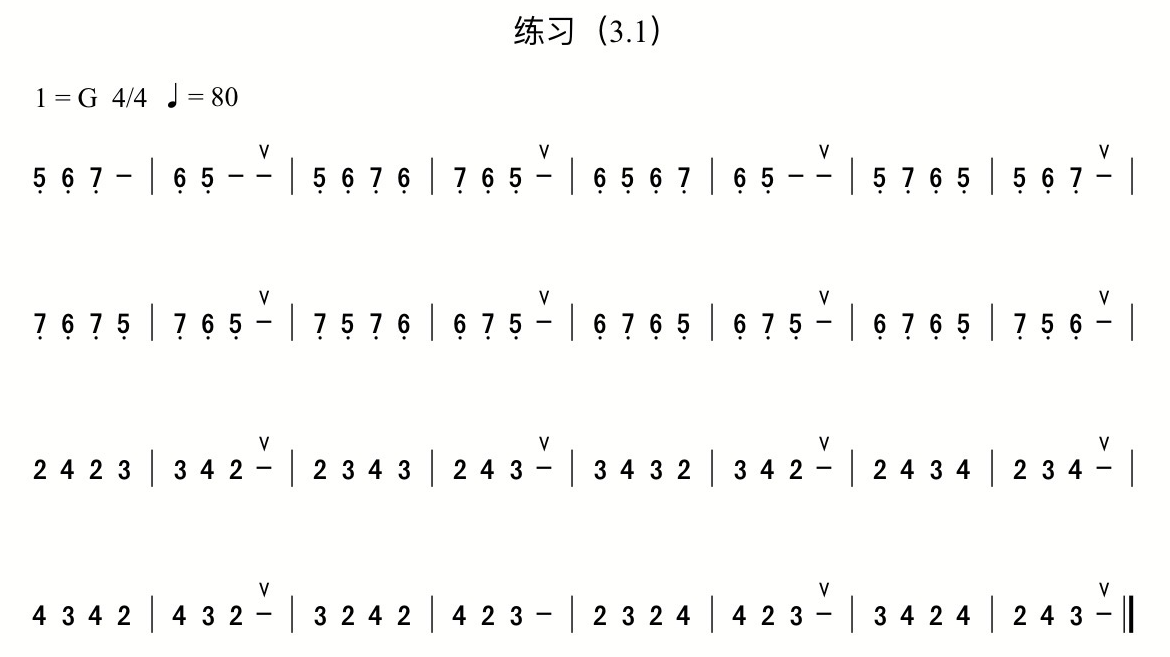
\includegraphics[width=\textwidth]{dongxiao/20200419-练习3.1.png}
\end{center}
\section{鐘聲}
	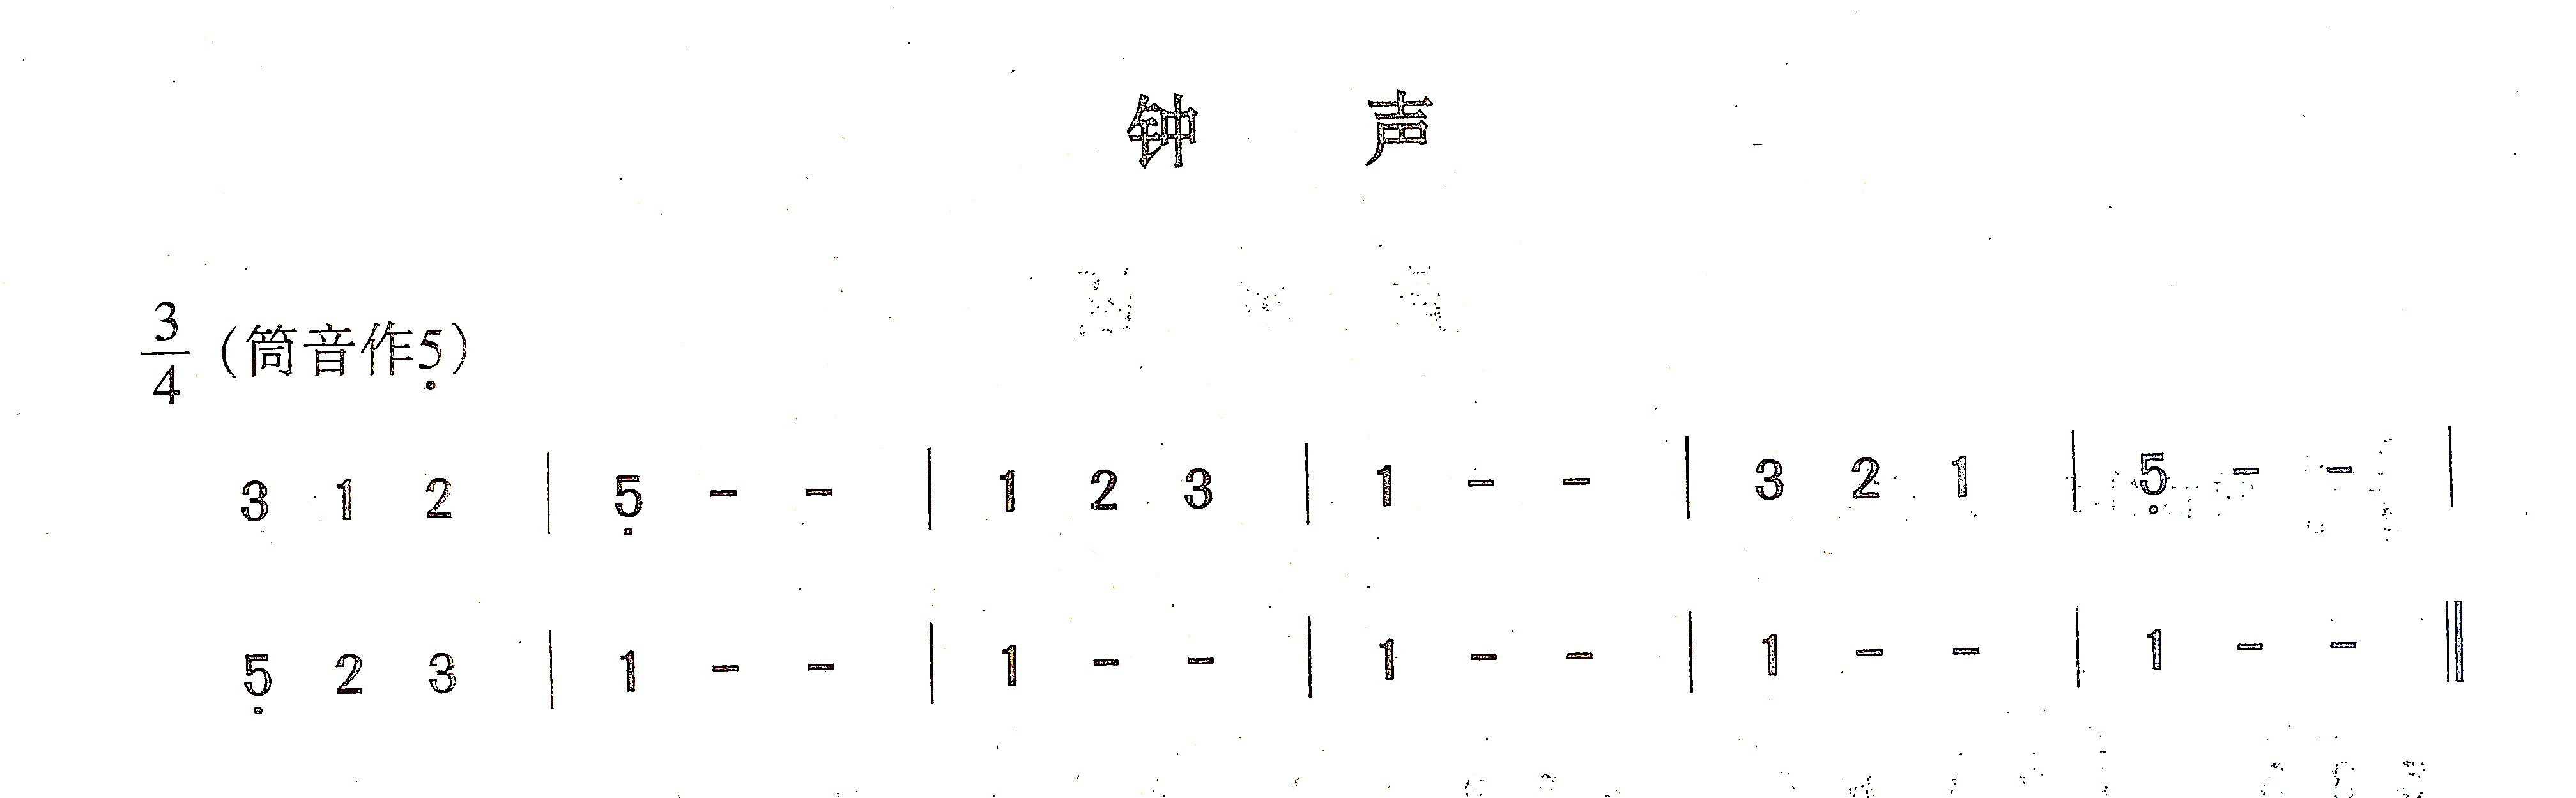
\includegraphics[width=\textwidth]{dongxiao/20200711-钟声.jpg}

\chapter{首选}
\section{静夜思}
    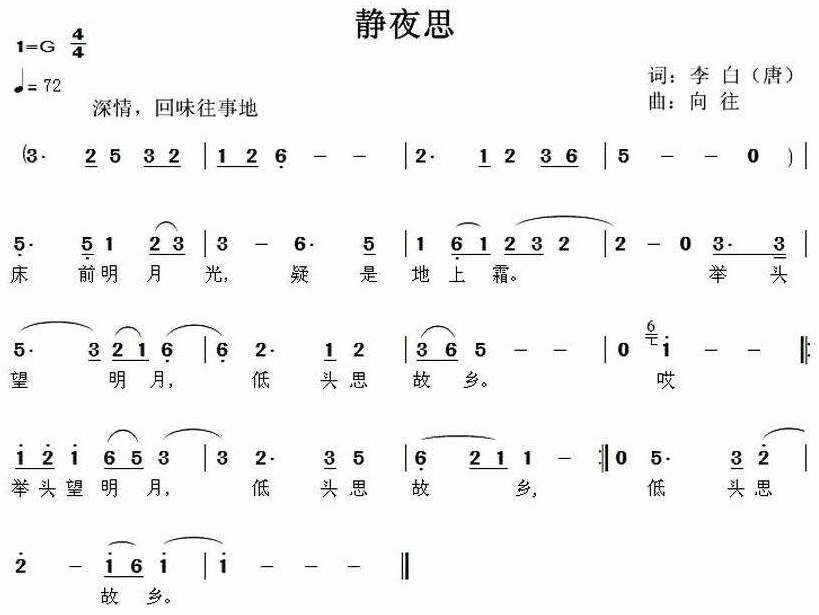
\includegraphics[width=0.9\textwidth]{dongxiao/20200411-静夜思}
\section{寒山僧蹤}
	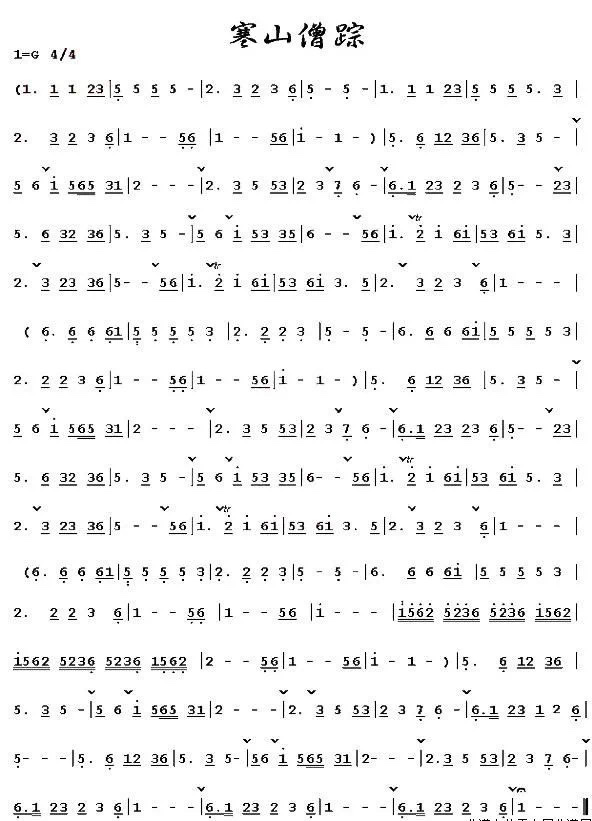
\includegraphics[width=0.95\textwidth]{dongxiao/20200926-寒山僧踪}  
\section{雪梅疏影}
    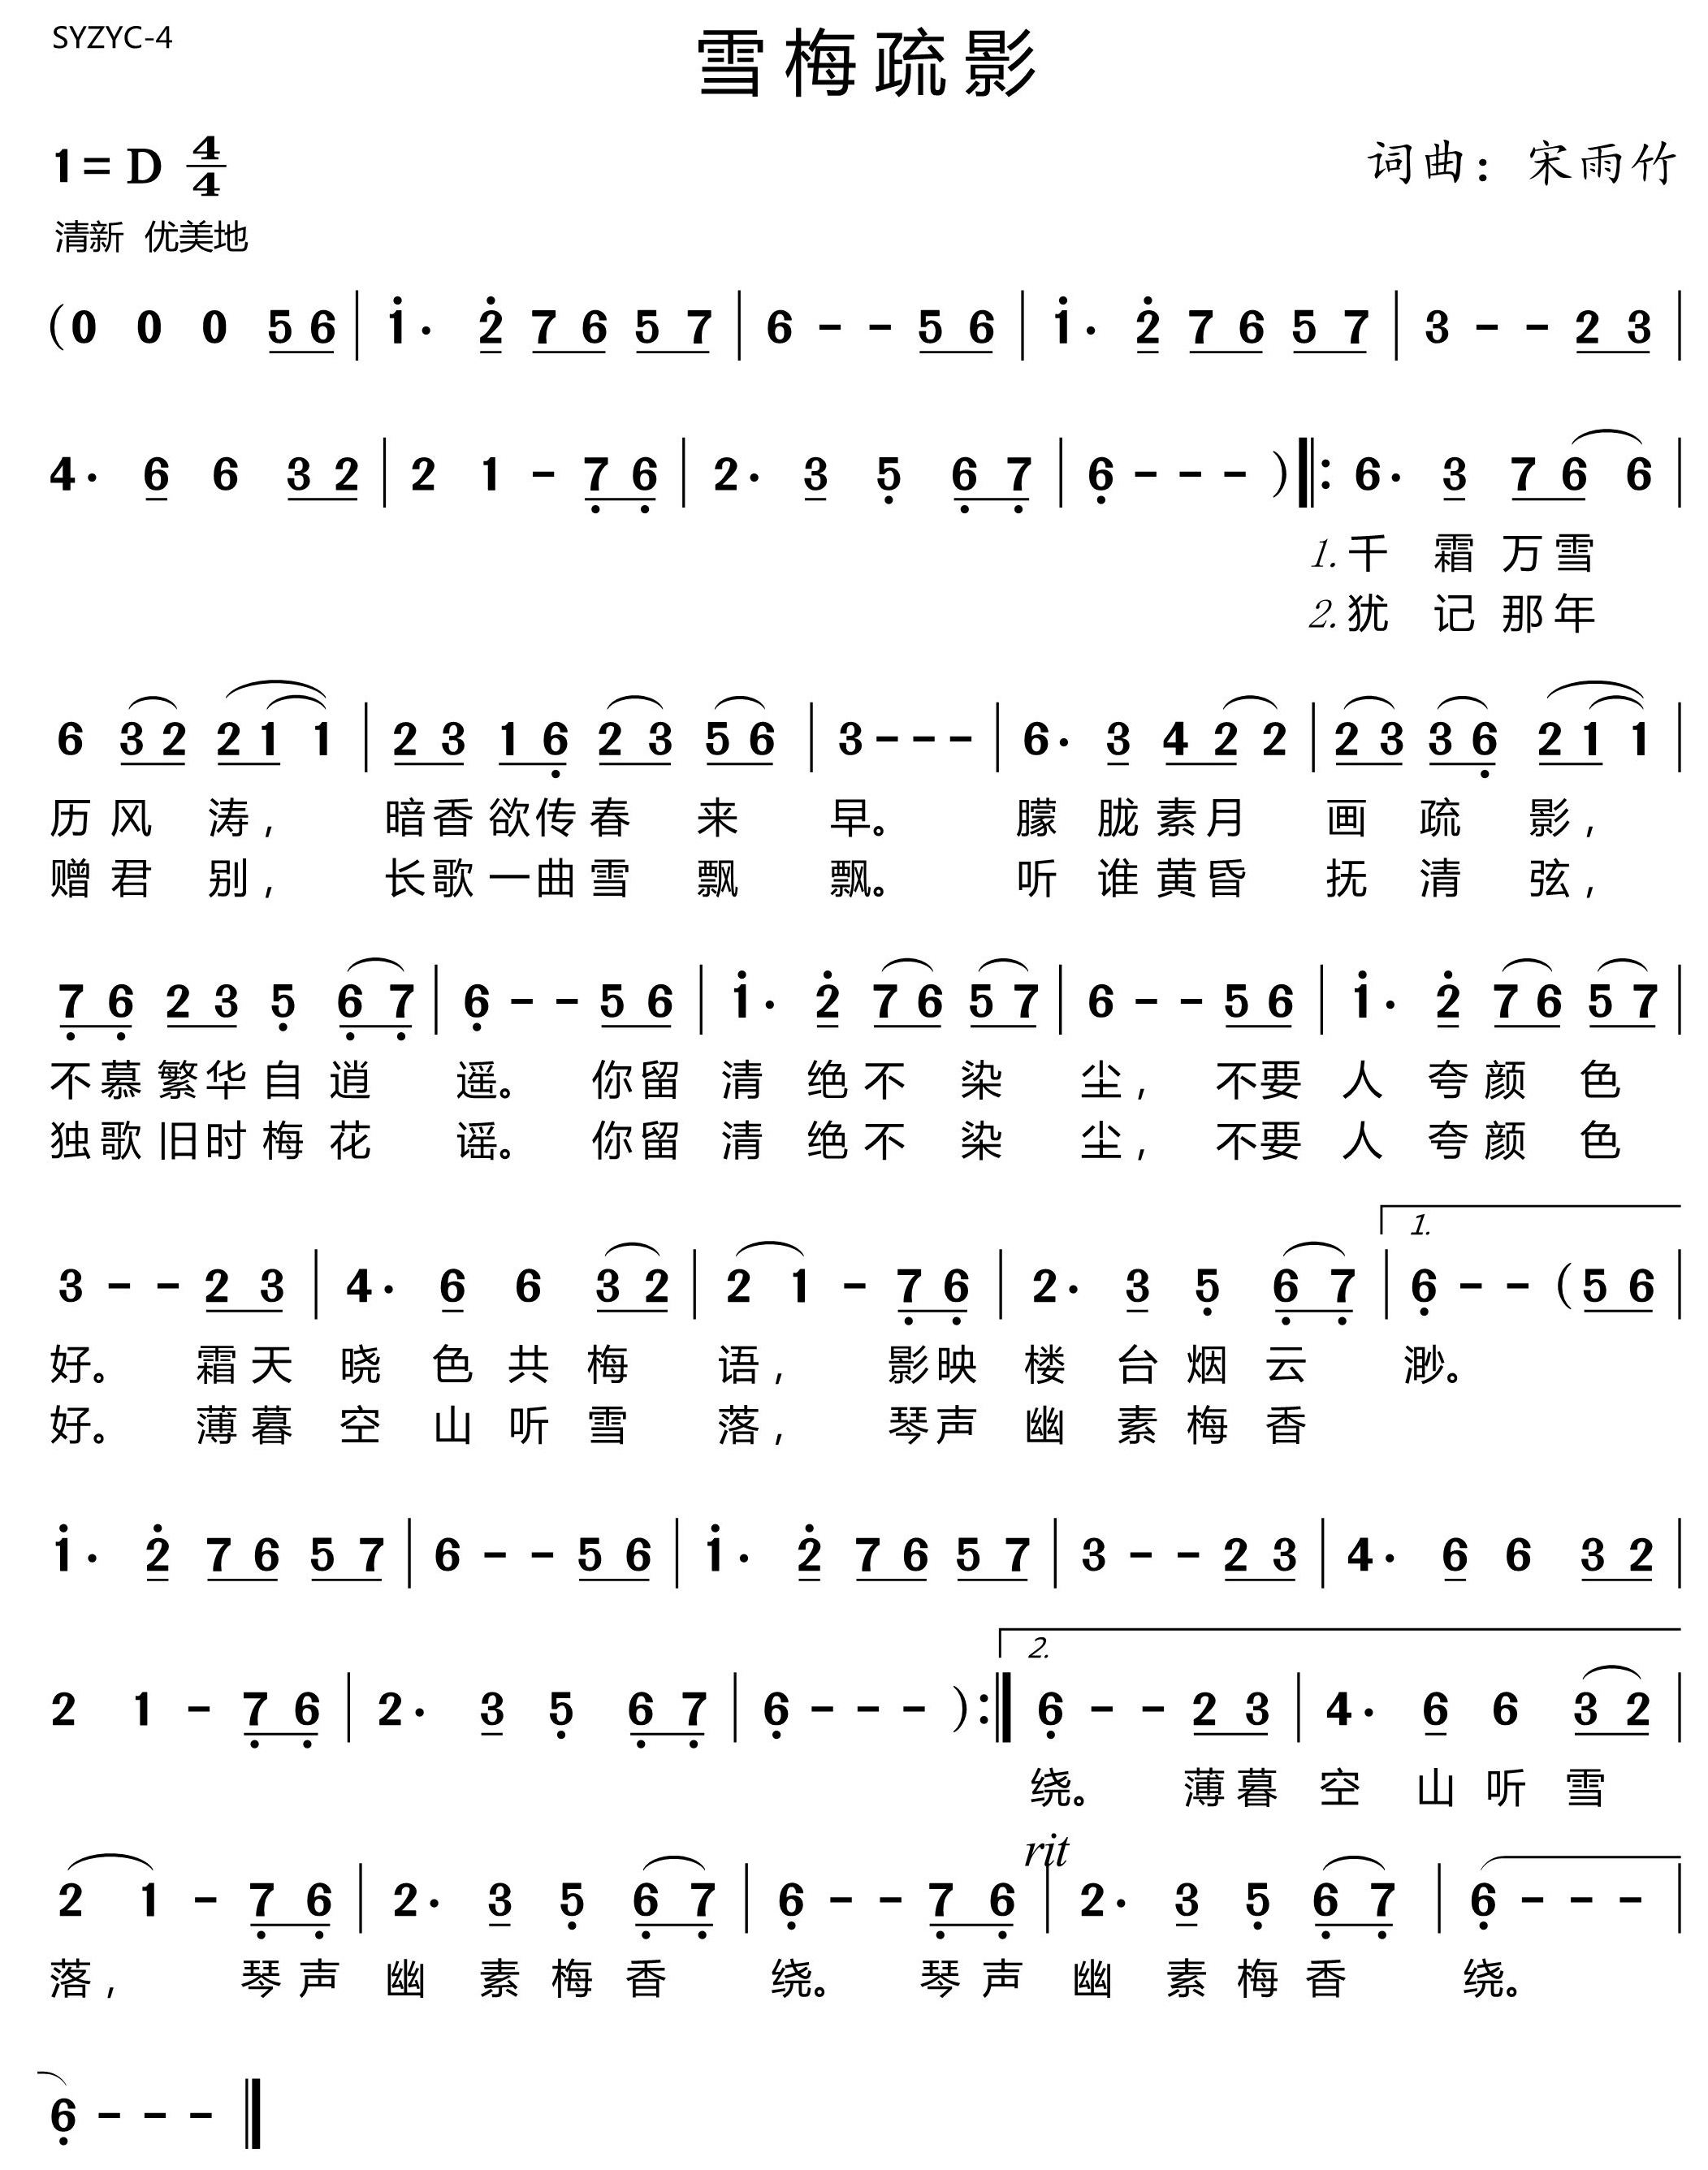
\includegraphics[width=0.9\textwidth]{dongxiao/20200725-雪梅疏影}
\section{时间都去哪儿了}
    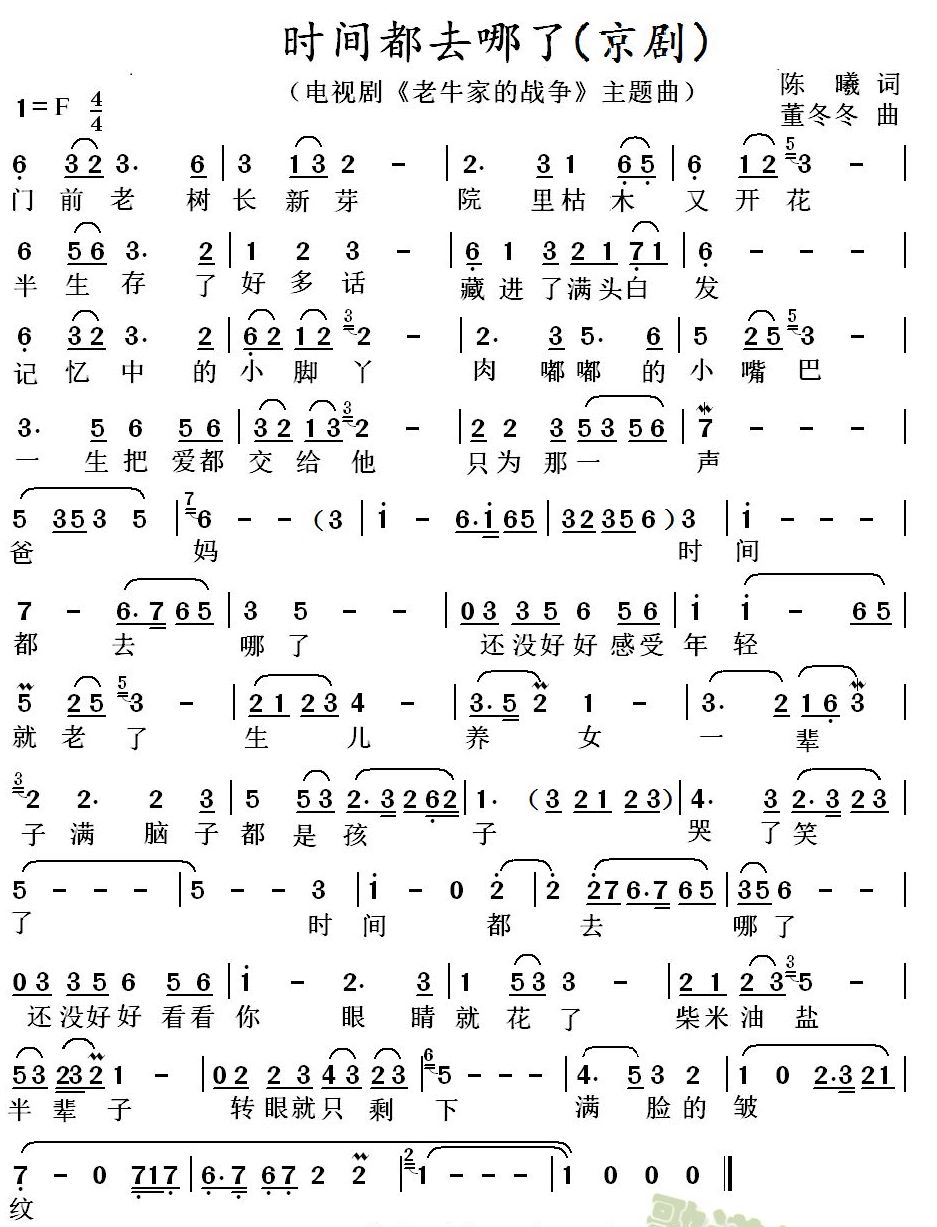
\includegraphics[width=\textwidth]{dongxiao/20200411-时间都去哪儿了.jpg}
                   
\chapter{西游记}
\section{西游记-敢问路在何方}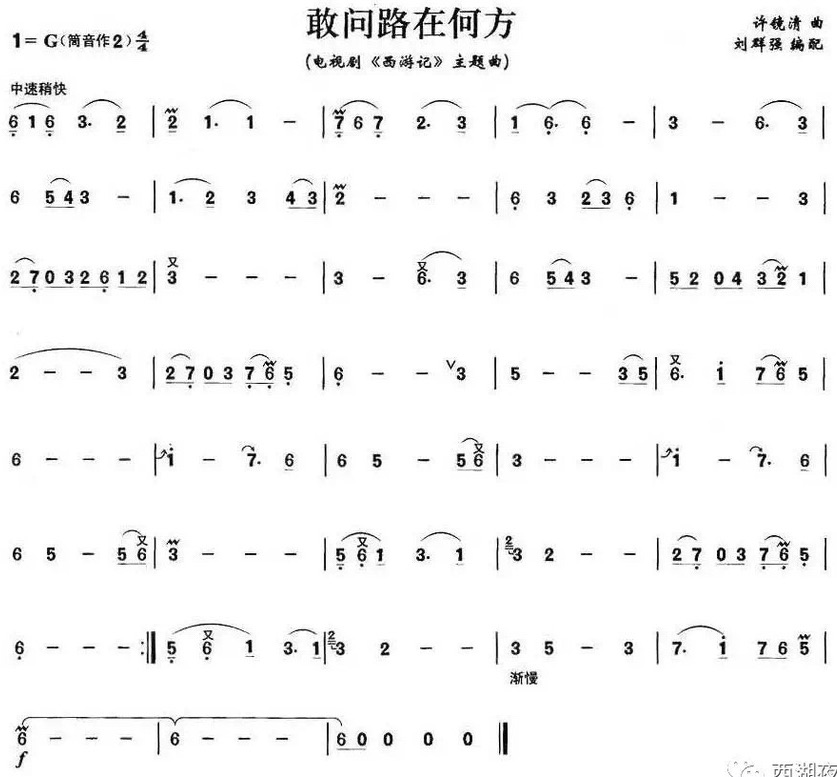
\includegraphics[width=\textwidth]{dongxiao/20200819/西游记-敢问路在何方.jpeg}
\section{女兒情}          
	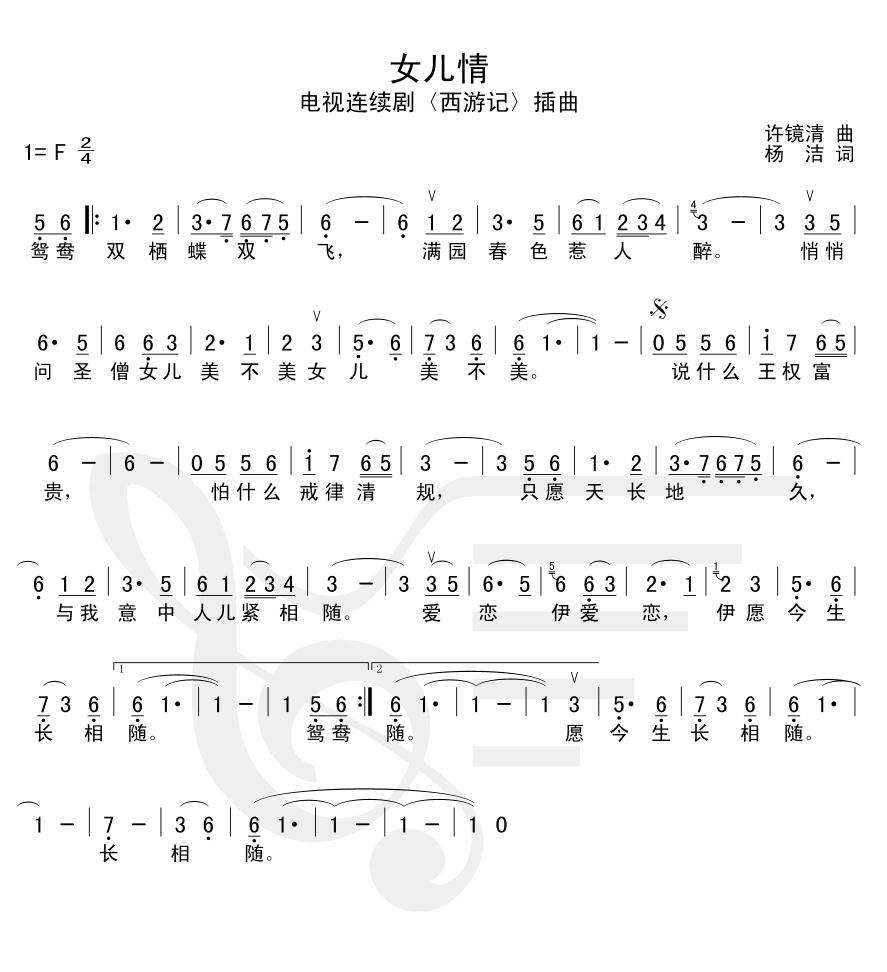
\includegraphics[width=\textwidth]{dongxiao/西游记-儿女情}  
	
\chapter{李叔同}
\section{忆儿时}
    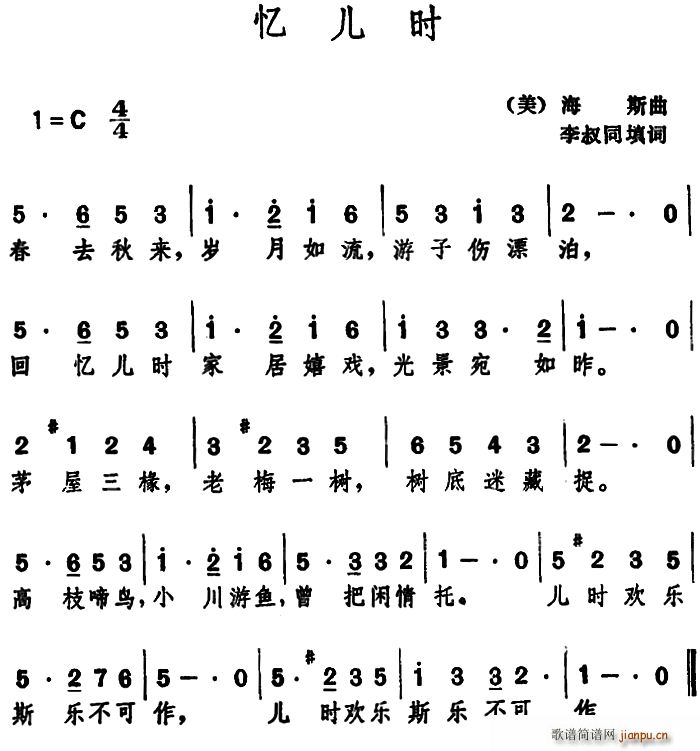
\includegraphics[width=\textwidth]{dongxiao/20200909-李叔同-忆儿时.jpg}  
\section{春游}
    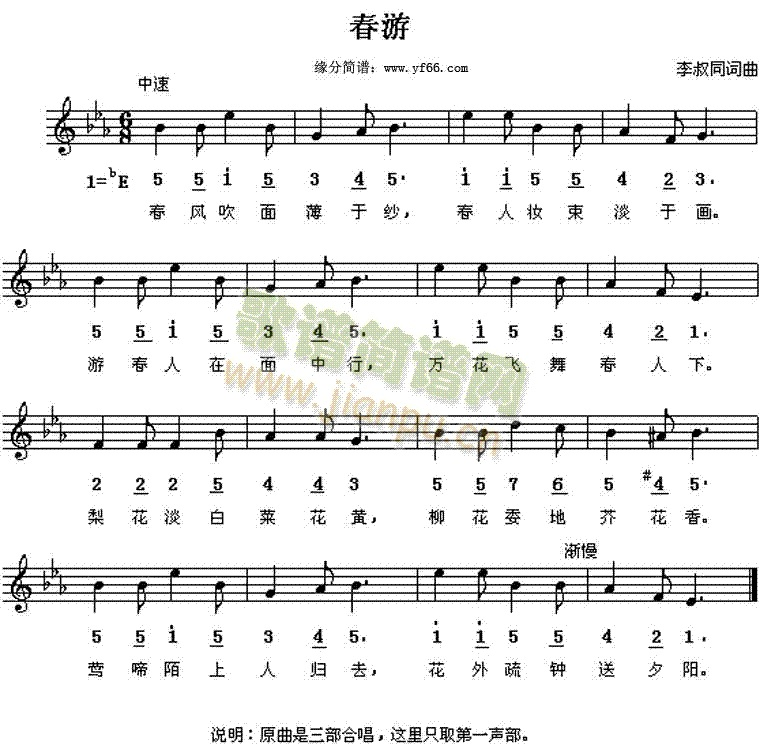
\includegraphics[width=\textwidth]{dongxiao/20200909-李叔同-春游.jpg} 
\section{早秋}
    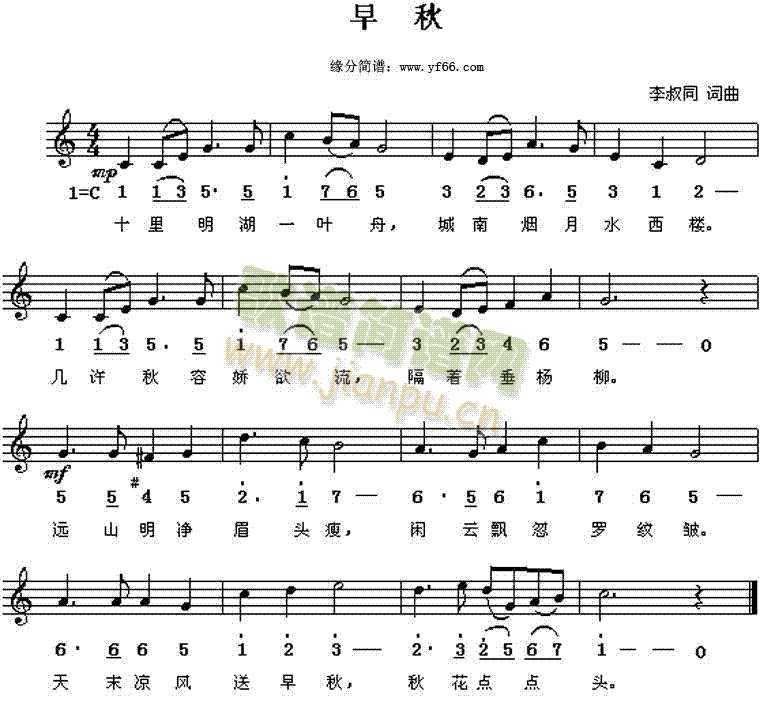
\includegraphics[width=\textwidth]{dongxiao/20200909-李叔同-早秋.jpg} 
\section{送别}
    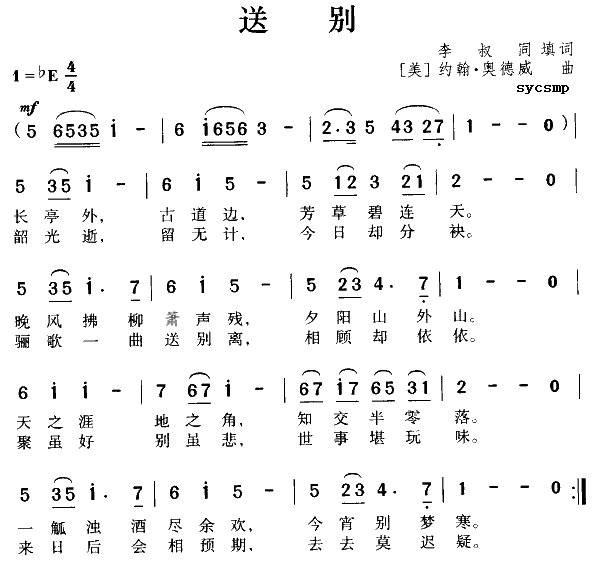
\includegraphics[width=\textwidth]{dongxiao/20200909-李叔同-送别.png} 

\chapter{王维}
\section{山中}
    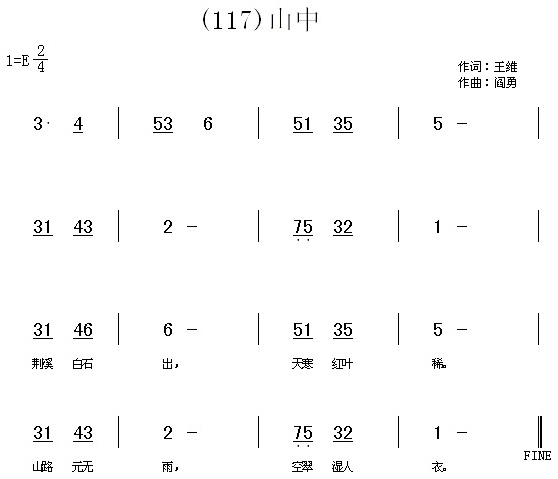
\includegraphics[width=\textwidth]{dongxiao/20200627-王维-山中.jpg}  
\section{\xpinyin*{山居秋暝}}
    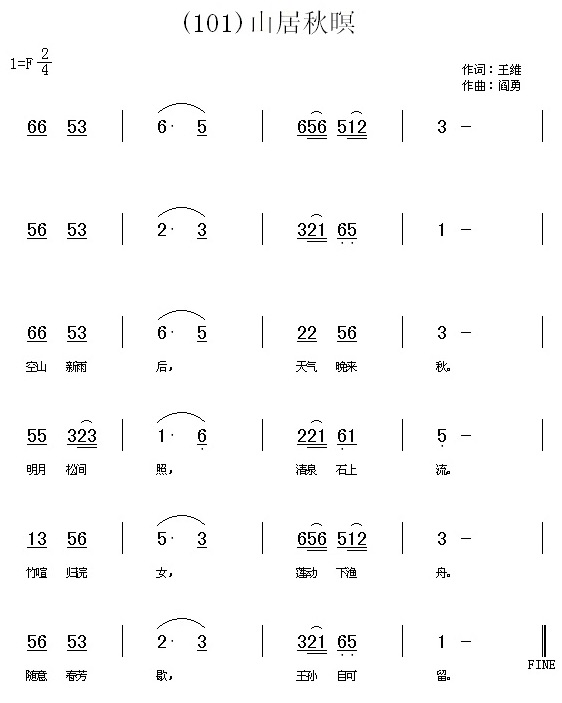
\includegraphics[width=\textwidth]{dongxiao/20200627-王维-山居秋暝.jpg} 
\section{辛夷坞}
    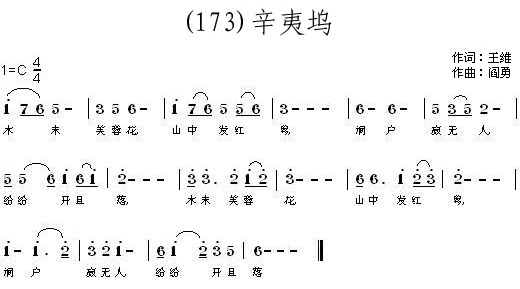
\includegraphics[width=\textwidth]{dongxiao/20200627-王维-辛夷坞.jpg} 

\chapter{曹操}
\section{短歌行}
    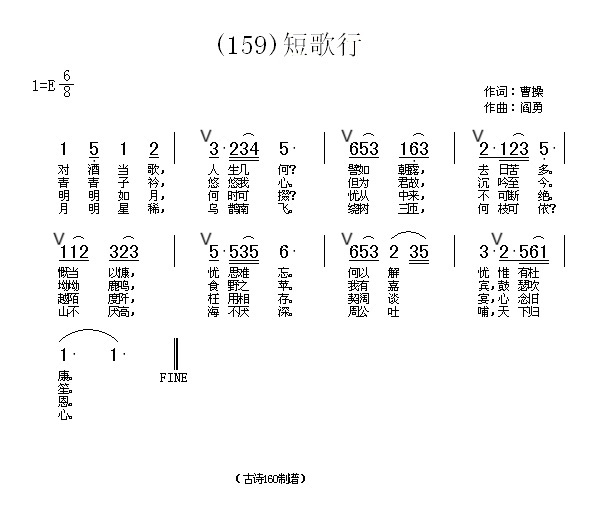
\includegraphics[width=\textwidth]{dongxiao/20200808-短歌行-曹操.jpg} 
\section{观沧海}
    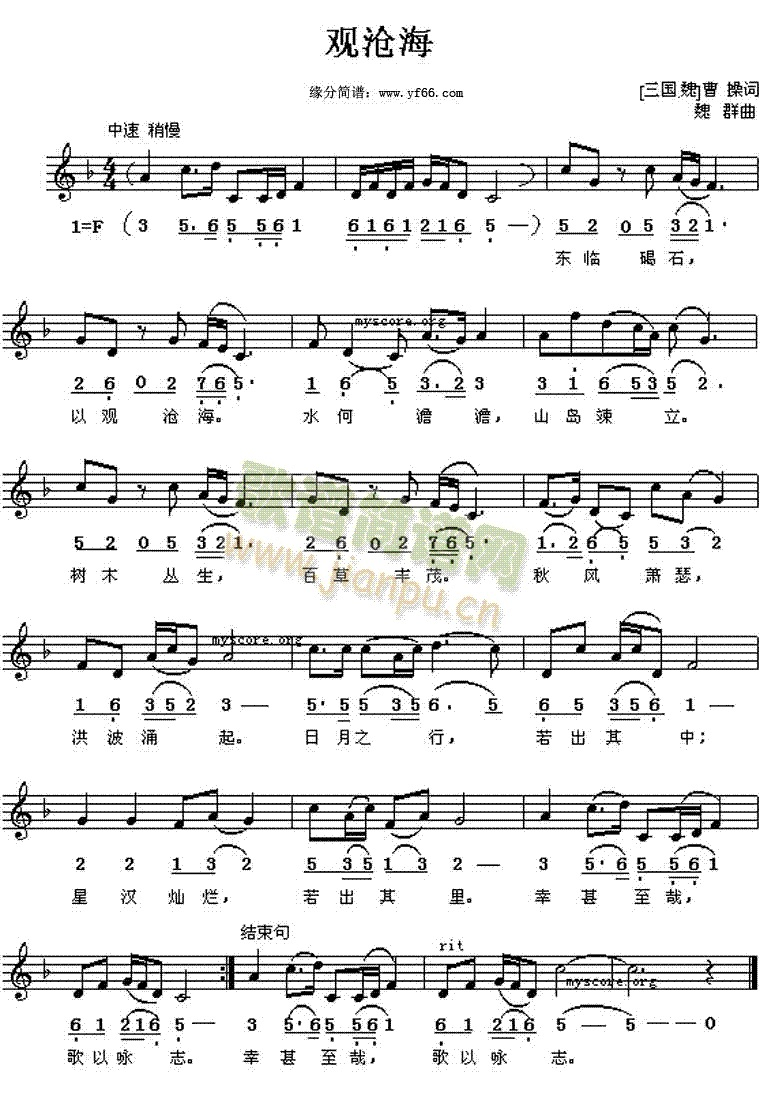
\includegraphics[width=0.9\textwidth]{dongxiao/20200808-观沧海-曹操.jpg}                             

\chapter{苏轼}
\section{黄州定慧院寓居作}
    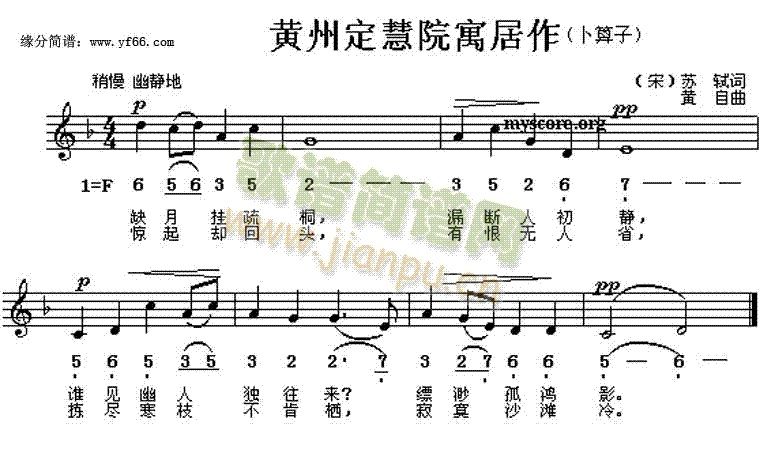
\includegraphics[width=\textwidth]{dongxiao/20200627-苏轼-黄州定慧院寓居作.jpg} 
\section{定风波}
    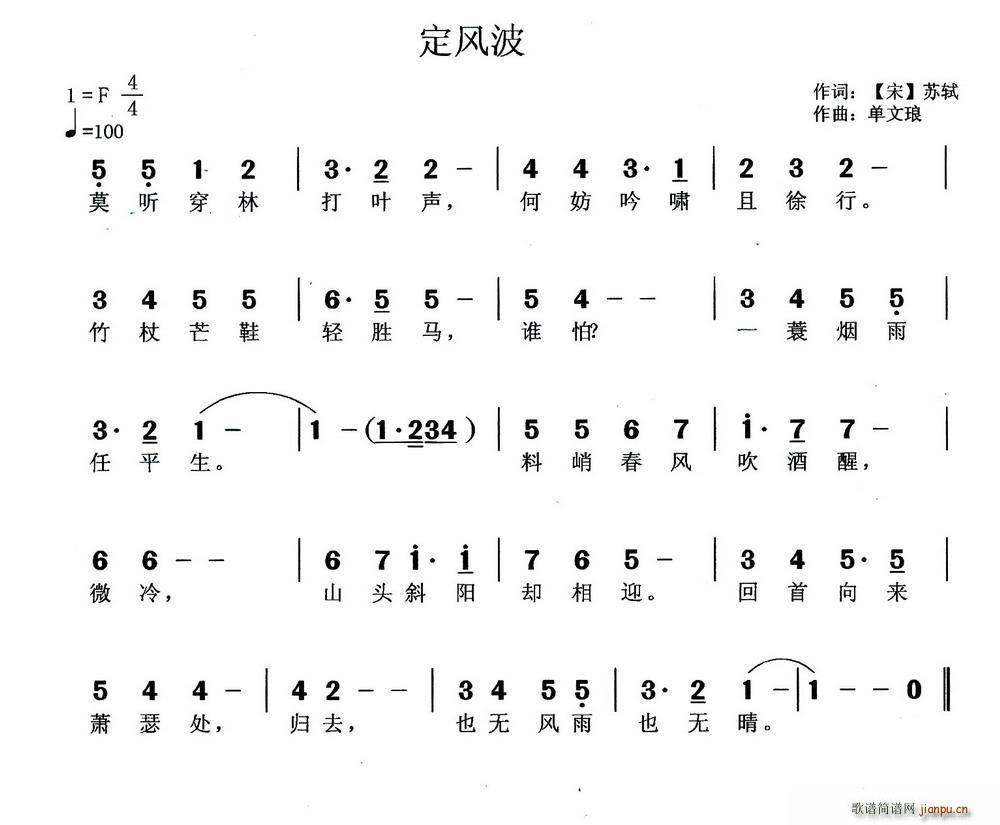
\includegraphics[width=\textwidth]{dongxiao/20200411-定风波.jpg}
\section{蝶恋花-春景}
    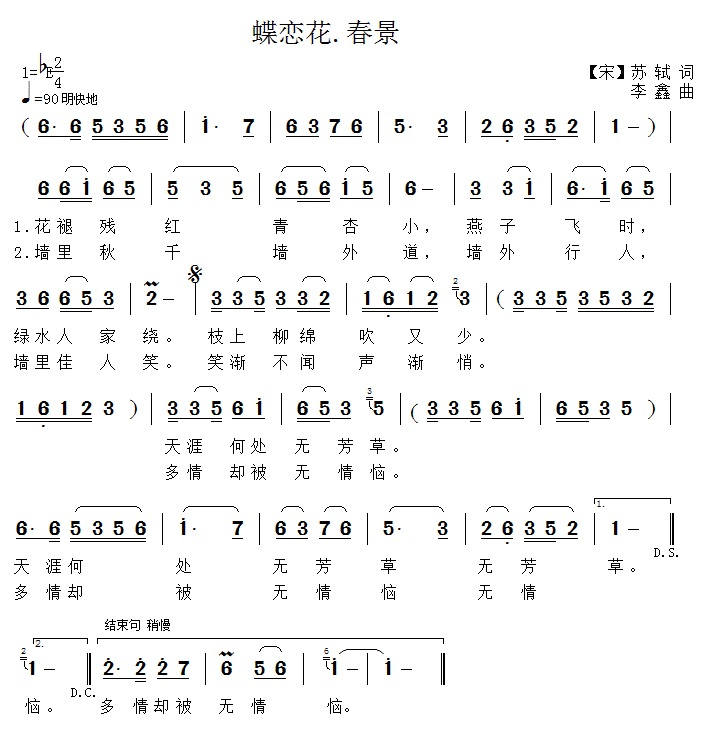
\includegraphics[width=\textwidth]{dongxiao/20200411-蝶恋花-春景.jpg}
\section{江城子}
    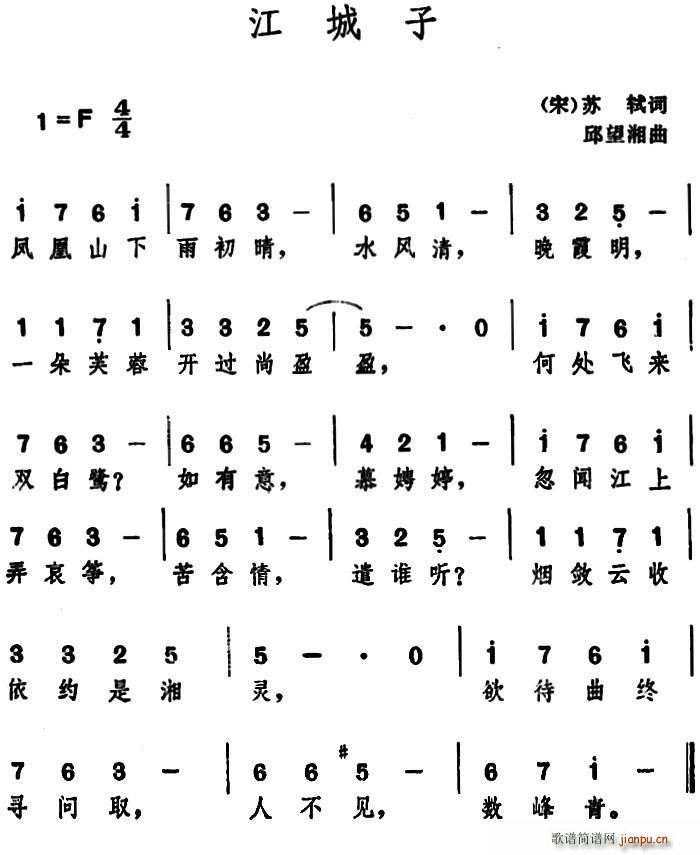
\includegraphics[width=\textwidth]{dongxiao/20200627-苏轼-江城子.jpg} 
\section{十年生死两茫茫}
    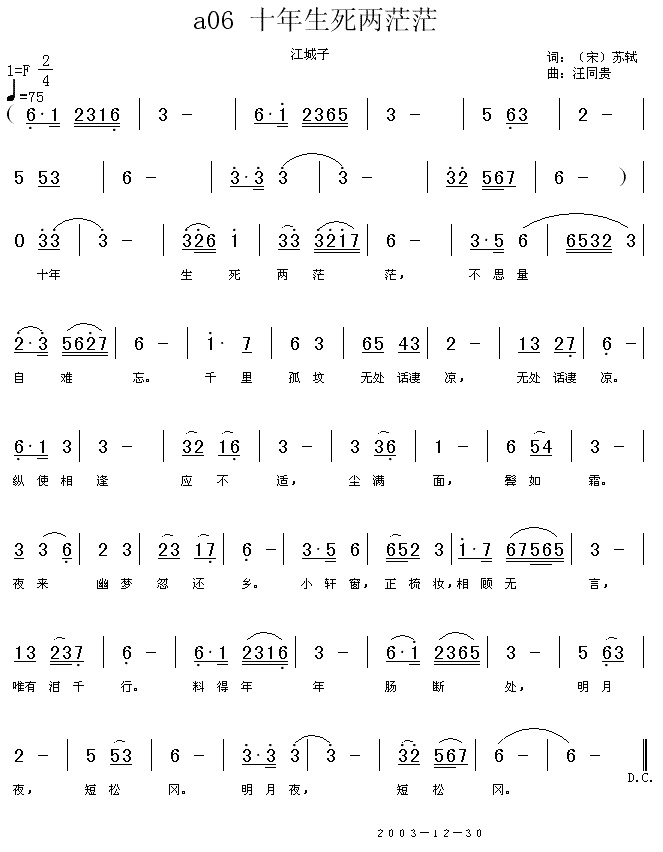
\includegraphics[width=\textwidth]{dongxiao/20200627-苏轼-十年生死两茫茫.jpg} 
\section{念奴娇赤壁怀古}
    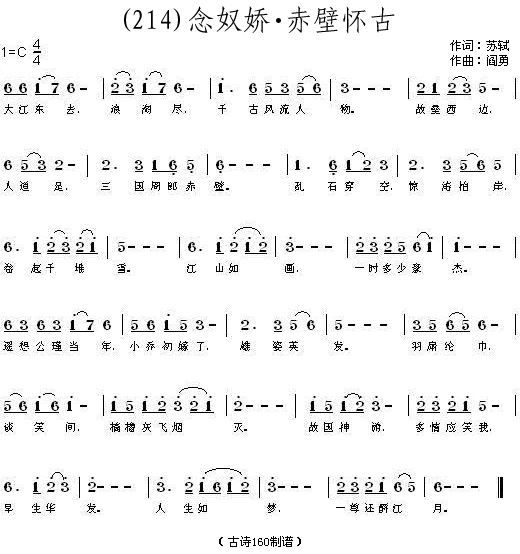
\includegraphics[width=\textwidth]{dongxiao/20200801-苏轼-念奴娇赤壁怀古}
   
\chapter{李清照}
\section{如梦令}
    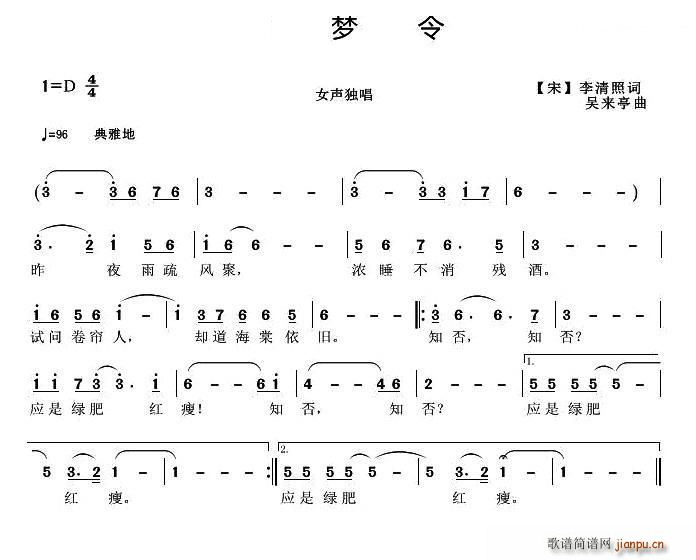
\includegraphics[width=\textwidth]{dongxiao/20200808-如梦令-李清照.jpg}
\section{昨夜雨疏风骤}
    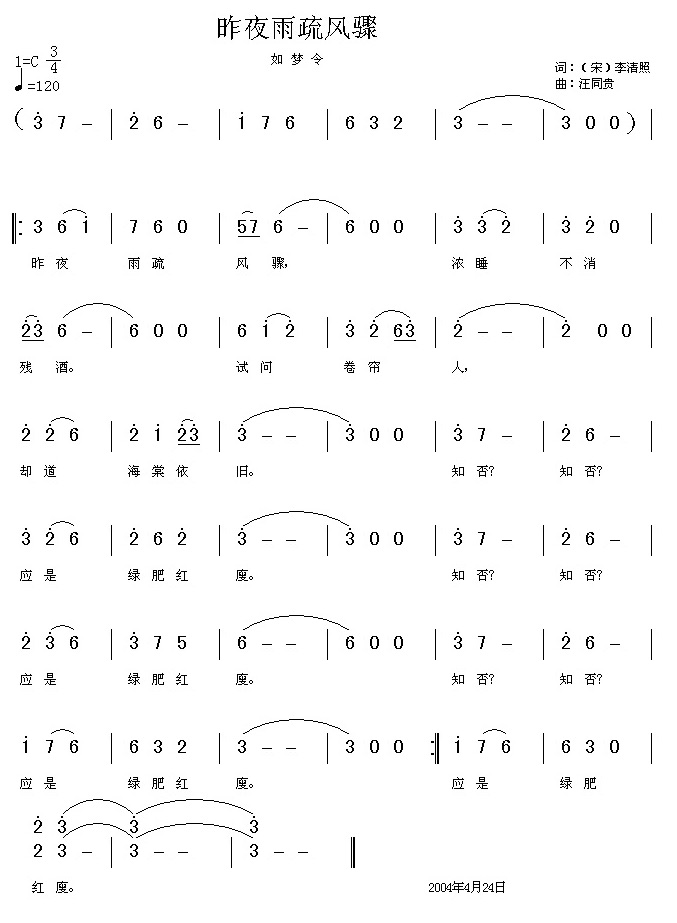
\includegraphics[width=\textwidth]{dongxiao/20200808-昨夜雨疏风骤-李清照.jpg}    
   
\chapter{杜甫}
\section{月夜}
    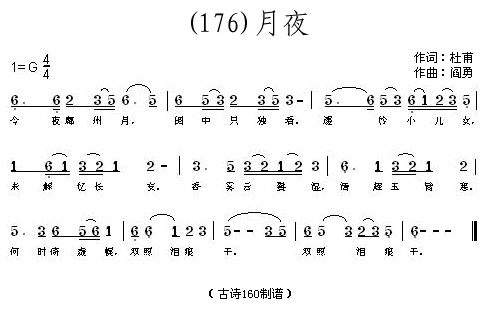
\includegraphics[width=\textwidth]{dongxiao/20200808-月夜-杜甫.jpg}  
\section{春夜喜雨}
    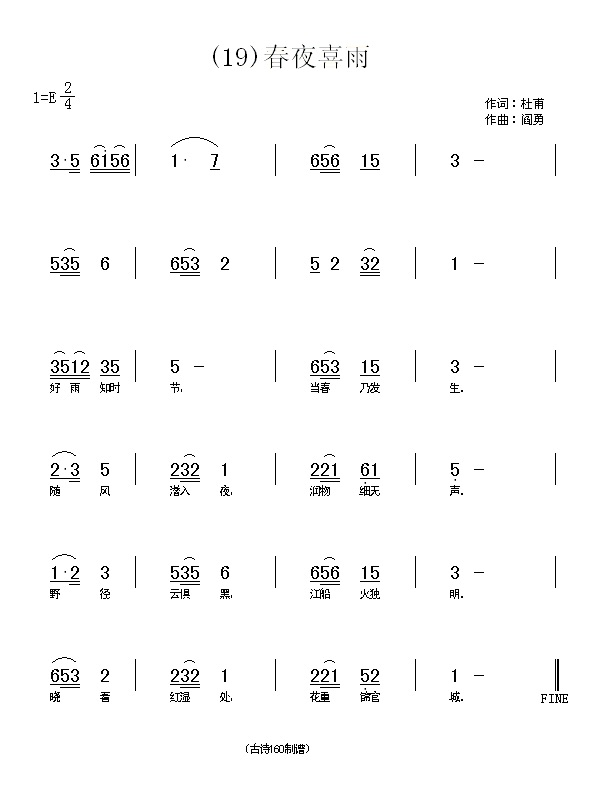
\includegraphics[width=0.9\textwidth]{dongxiao/20200808-春夜喜雨-杜甫.jpg}
                   
  

\chapter{李白}
\section{忆秦娥}
    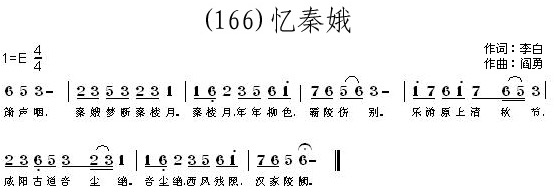
\includegraphics[width=\textwidth]{dongxiao/20200808-忆秦娥-李白.jpg} 
\section{菩萨蛮}
    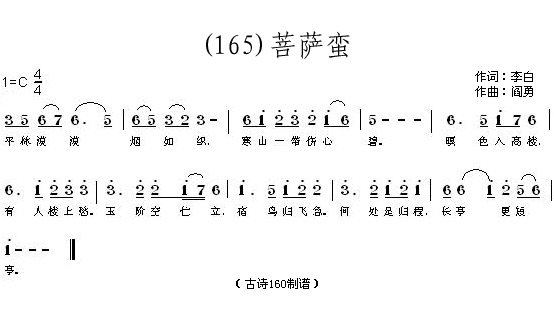
\includegraphics[width=\textwidth]{dongxiao/20200808-菩萨蛮-李白.jpg} 
\section{菩萨蛮.箫声咽}
    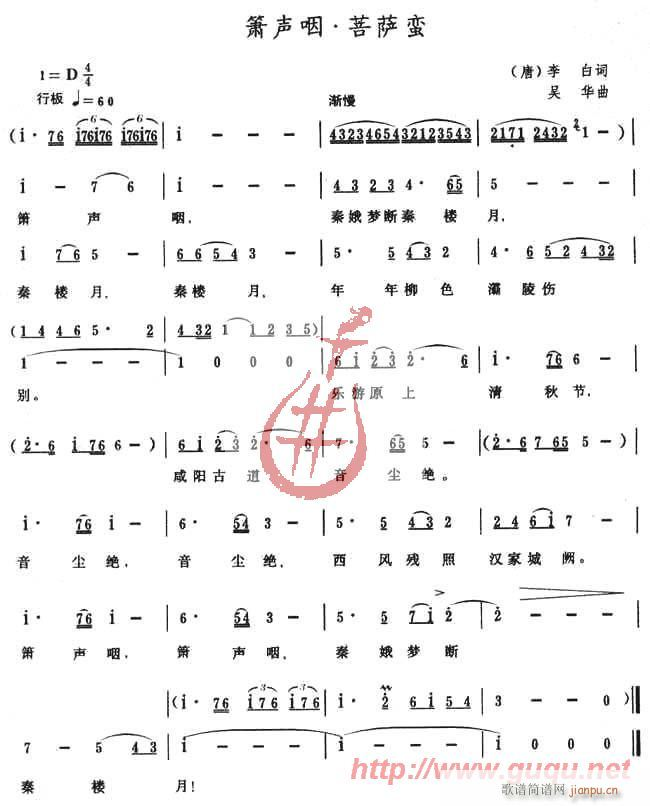
\includegraphics[width=0.95\textwidth]{dongxiao/20200909-箫声咽-菩萨蛮.jpg}
\section{美人怨}
    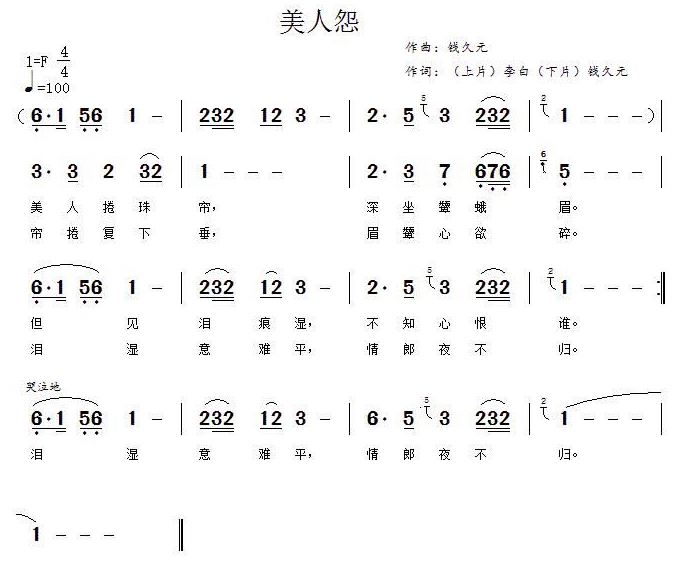
\includegraphics[width=\textwidth]{dongxiao/20200808-美人怨-李白.jpg}

      
\chapter{陆游}
\section{题临安邸}
    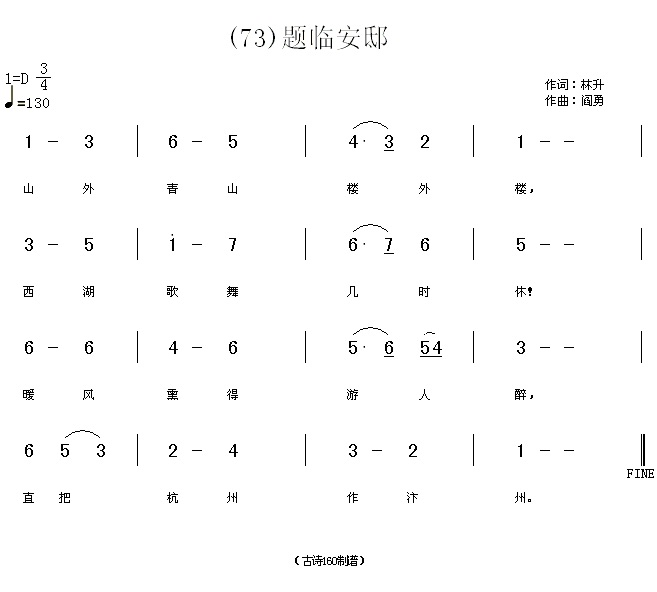
\includegraphics[width=\textwidth]{dongxiao/20200808-题临安邸-陆游.jpg}
\section{钗头凤}
    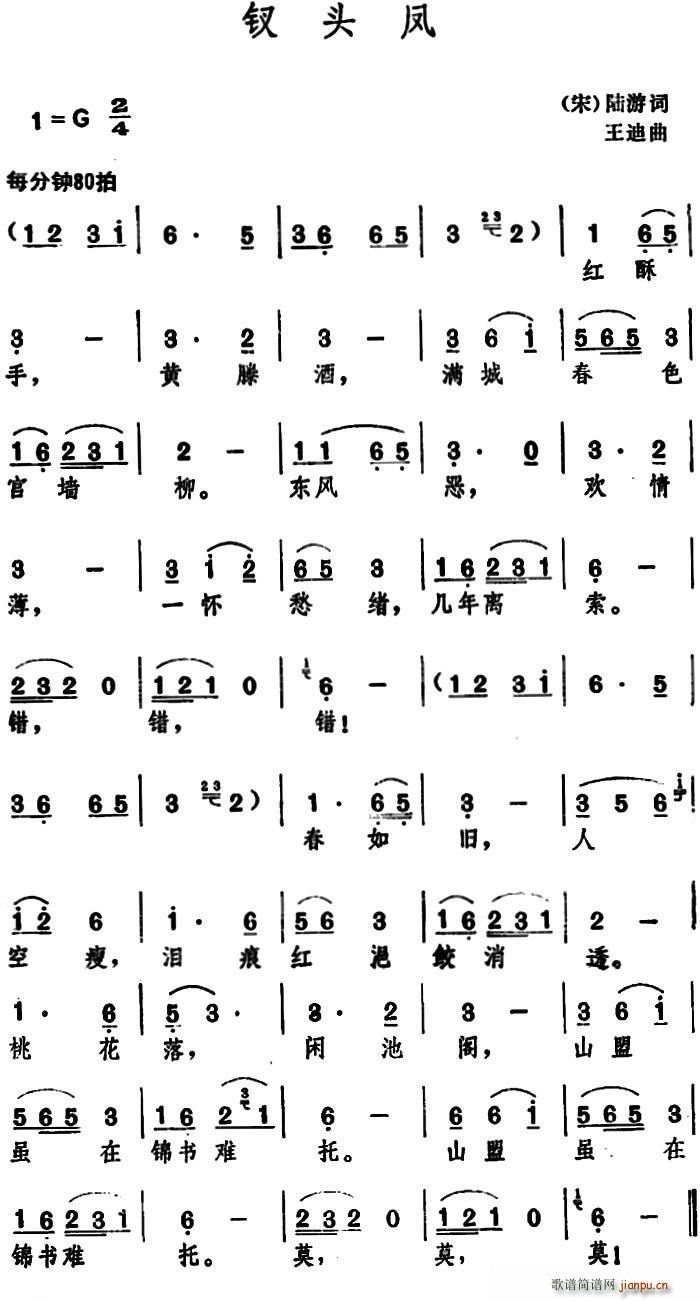
\includegraphics[width=0.7\textwidth]{dongxiao/20200808-钗头凤-陆游.jpg}                             
                             
 
\chapter{古诗}  
\section{枫桥夜泊}
    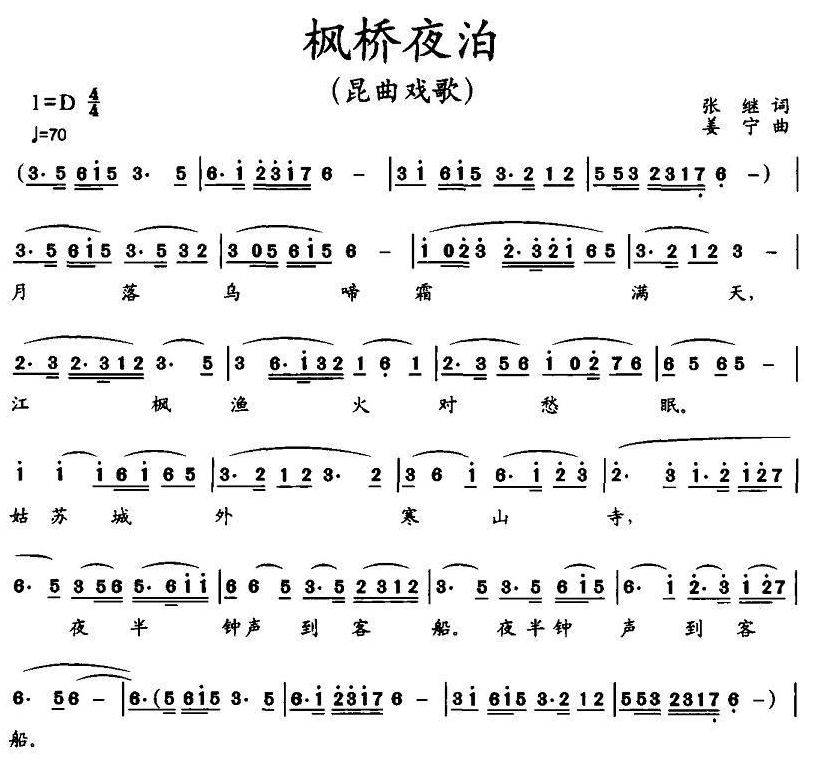
\includegraphics[width=\textwidth]{dongxiao/20200808-枫桥夜泊-昆曲.jpg}   
\section{枫桥夜泊2}
    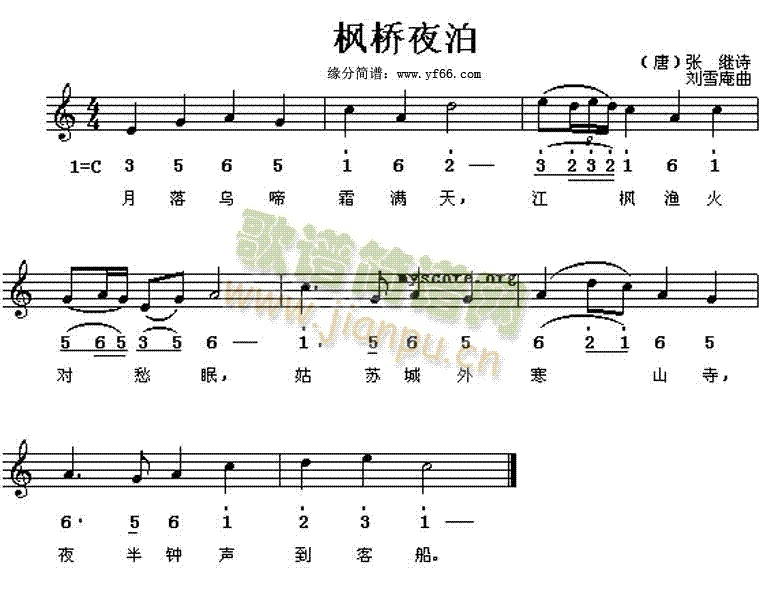
\includegraphics[width=\textwidth]{dongxiao/20200808-枫桥夜泊-张继.jpg}  
\section{七步诗}
    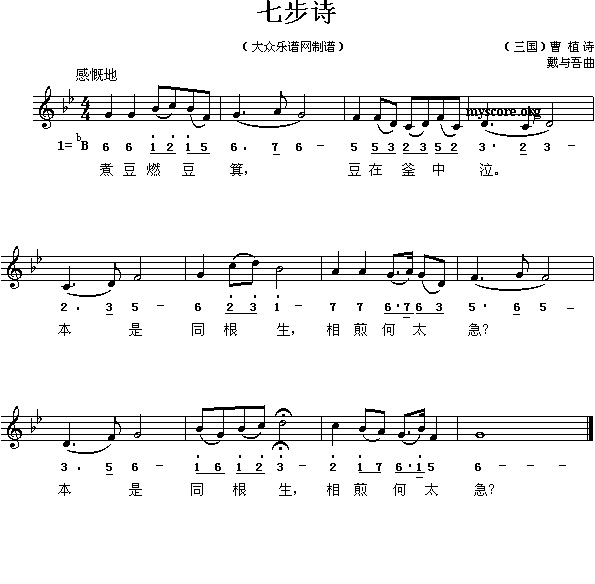
\includegraphics[width=\textwidth]{dongxiao/20200808-七步诗-戴与吾.jpg}
\section{七步诗2}
    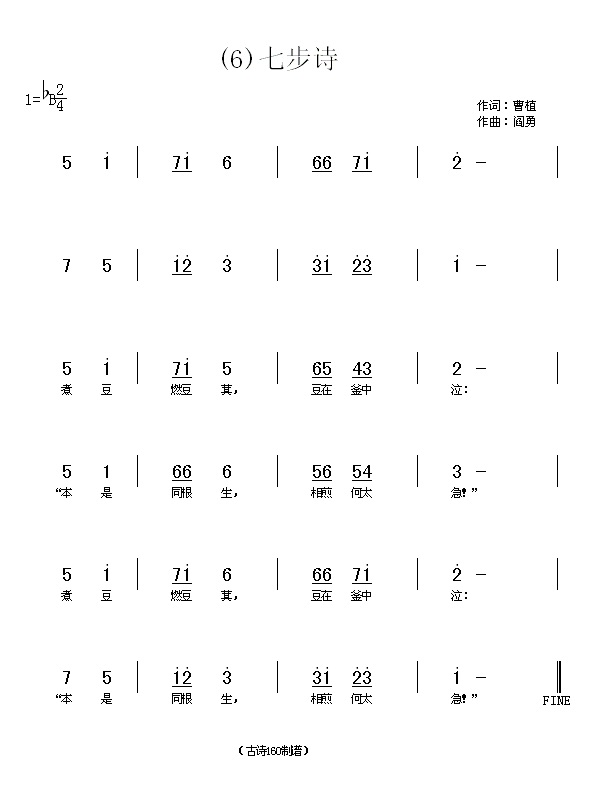
\includegraphics[width=\textwidth]{dongxiao/20200808-七步诗-曹植.jpg}
\section{饮酒}
    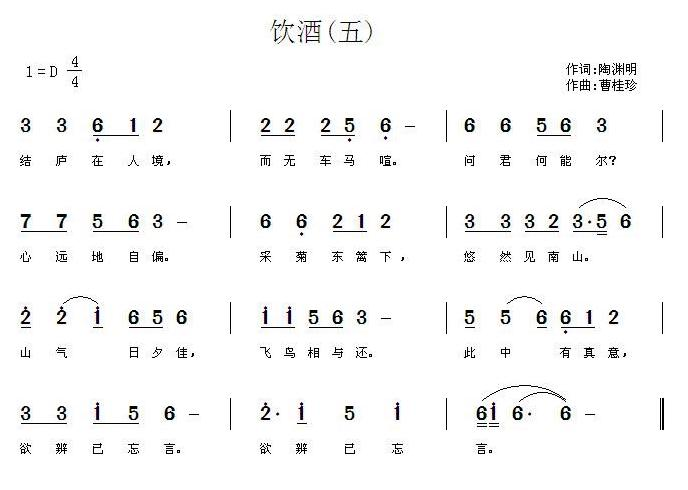
\includegraphics[width=\textwidth]{dongxiao/20200808-饮酒-陶渊明.jpg}
\section{浪淘沙}
    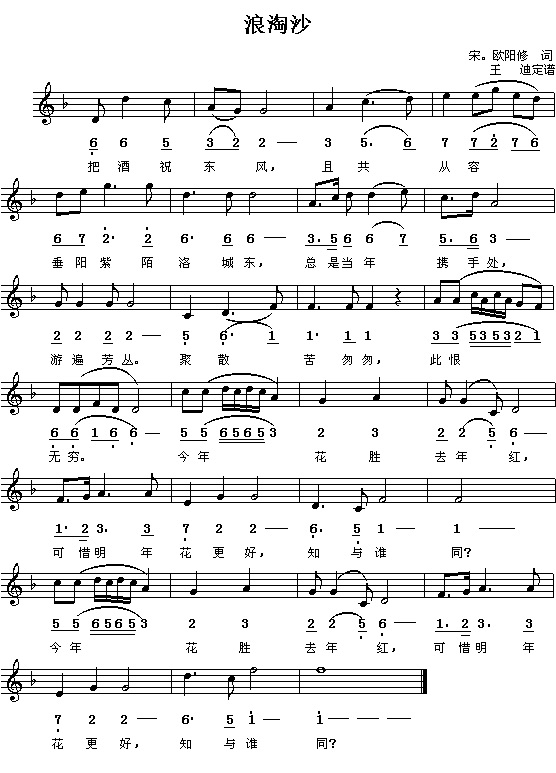
\includegraphics[width=0.95\textwidth]{dongxiao/20200808-浪淘沙-欧阳修.jpg}
\section{渔舟唱晚}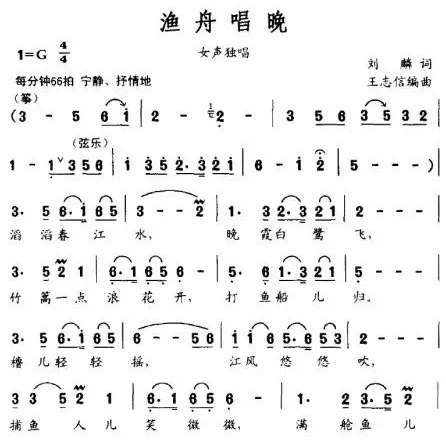
\includegraphics[width=\textwidth]{dongxiao/20200819/渔舟唱晚.jpeg}
\section{乌衣巷}
    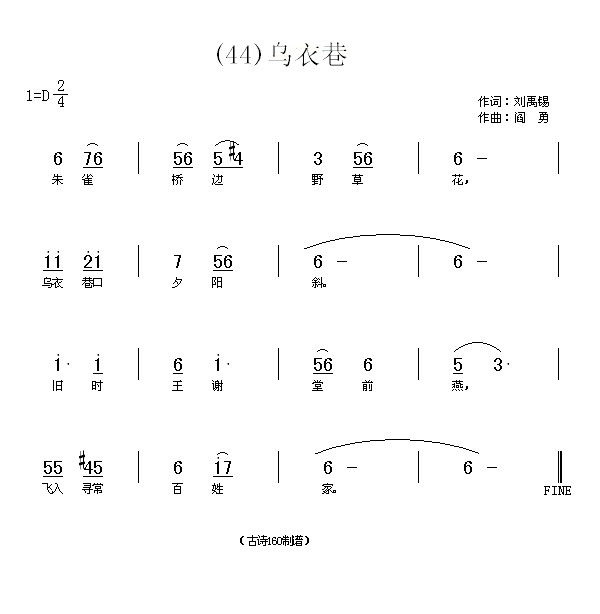
\includegraphics[width=\textwidth]{dongxiao/20200808-乌衣巷-刘禹锡.jpg}
\section{关山月}
    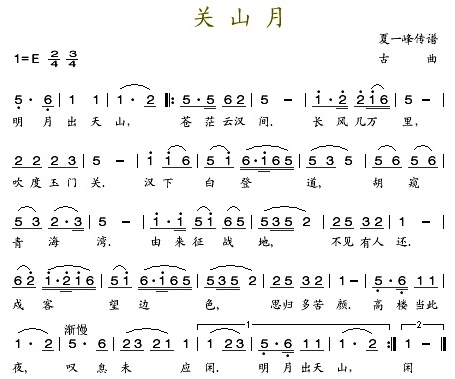
\includegraphics[width=\textwidth]{dongxiao/20200411-清平乐-关山月.jpg}
\section{清平乐-春归何处}
    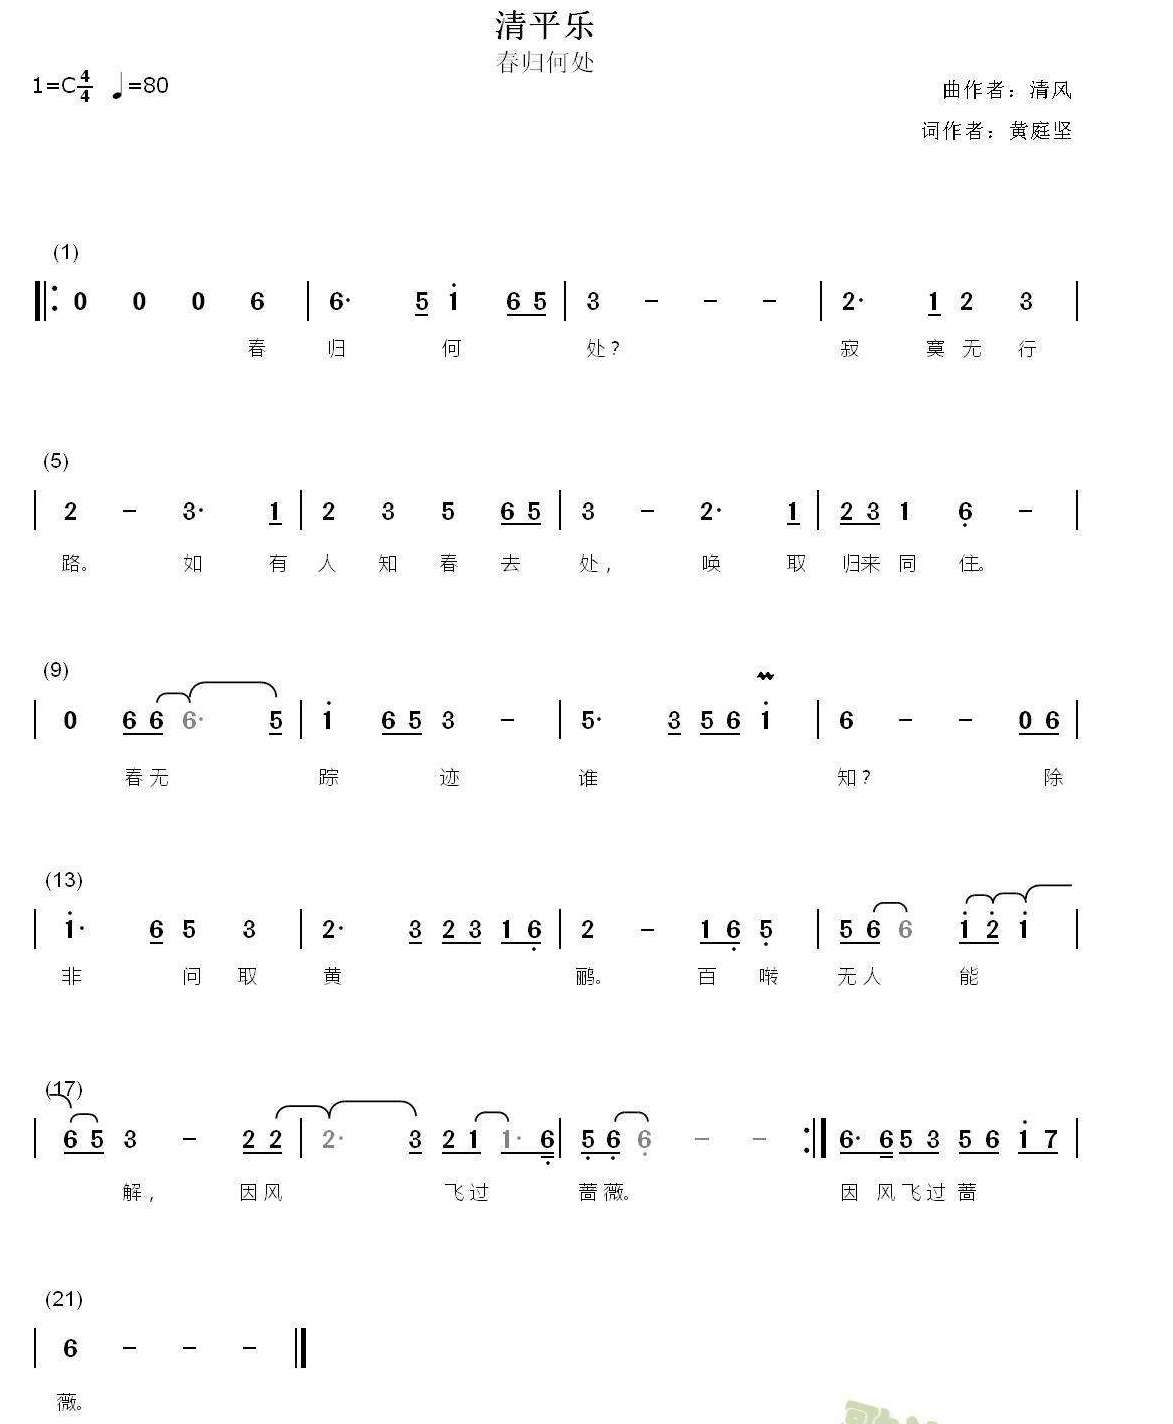
\includegraphics[width=\textwidth]{dongxiao/20200411-清平乐-春归何处.jpg}
\section{清平乐-晏殊词}
    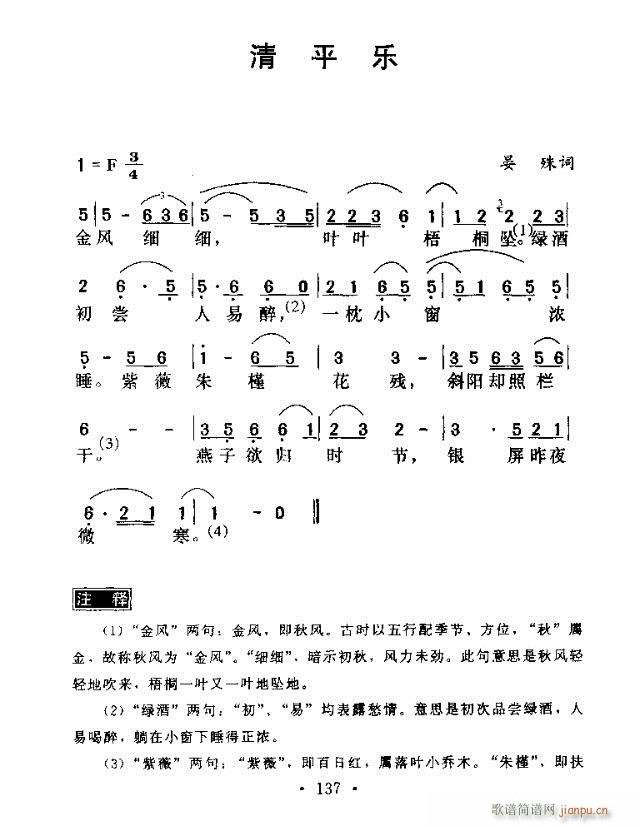
\includegraphics[width=\textwidth]{dongxiao/20200411-清平乐-晏殊.jpg}
                      
\chapter{雜谱錄}
\section{长城谣}
    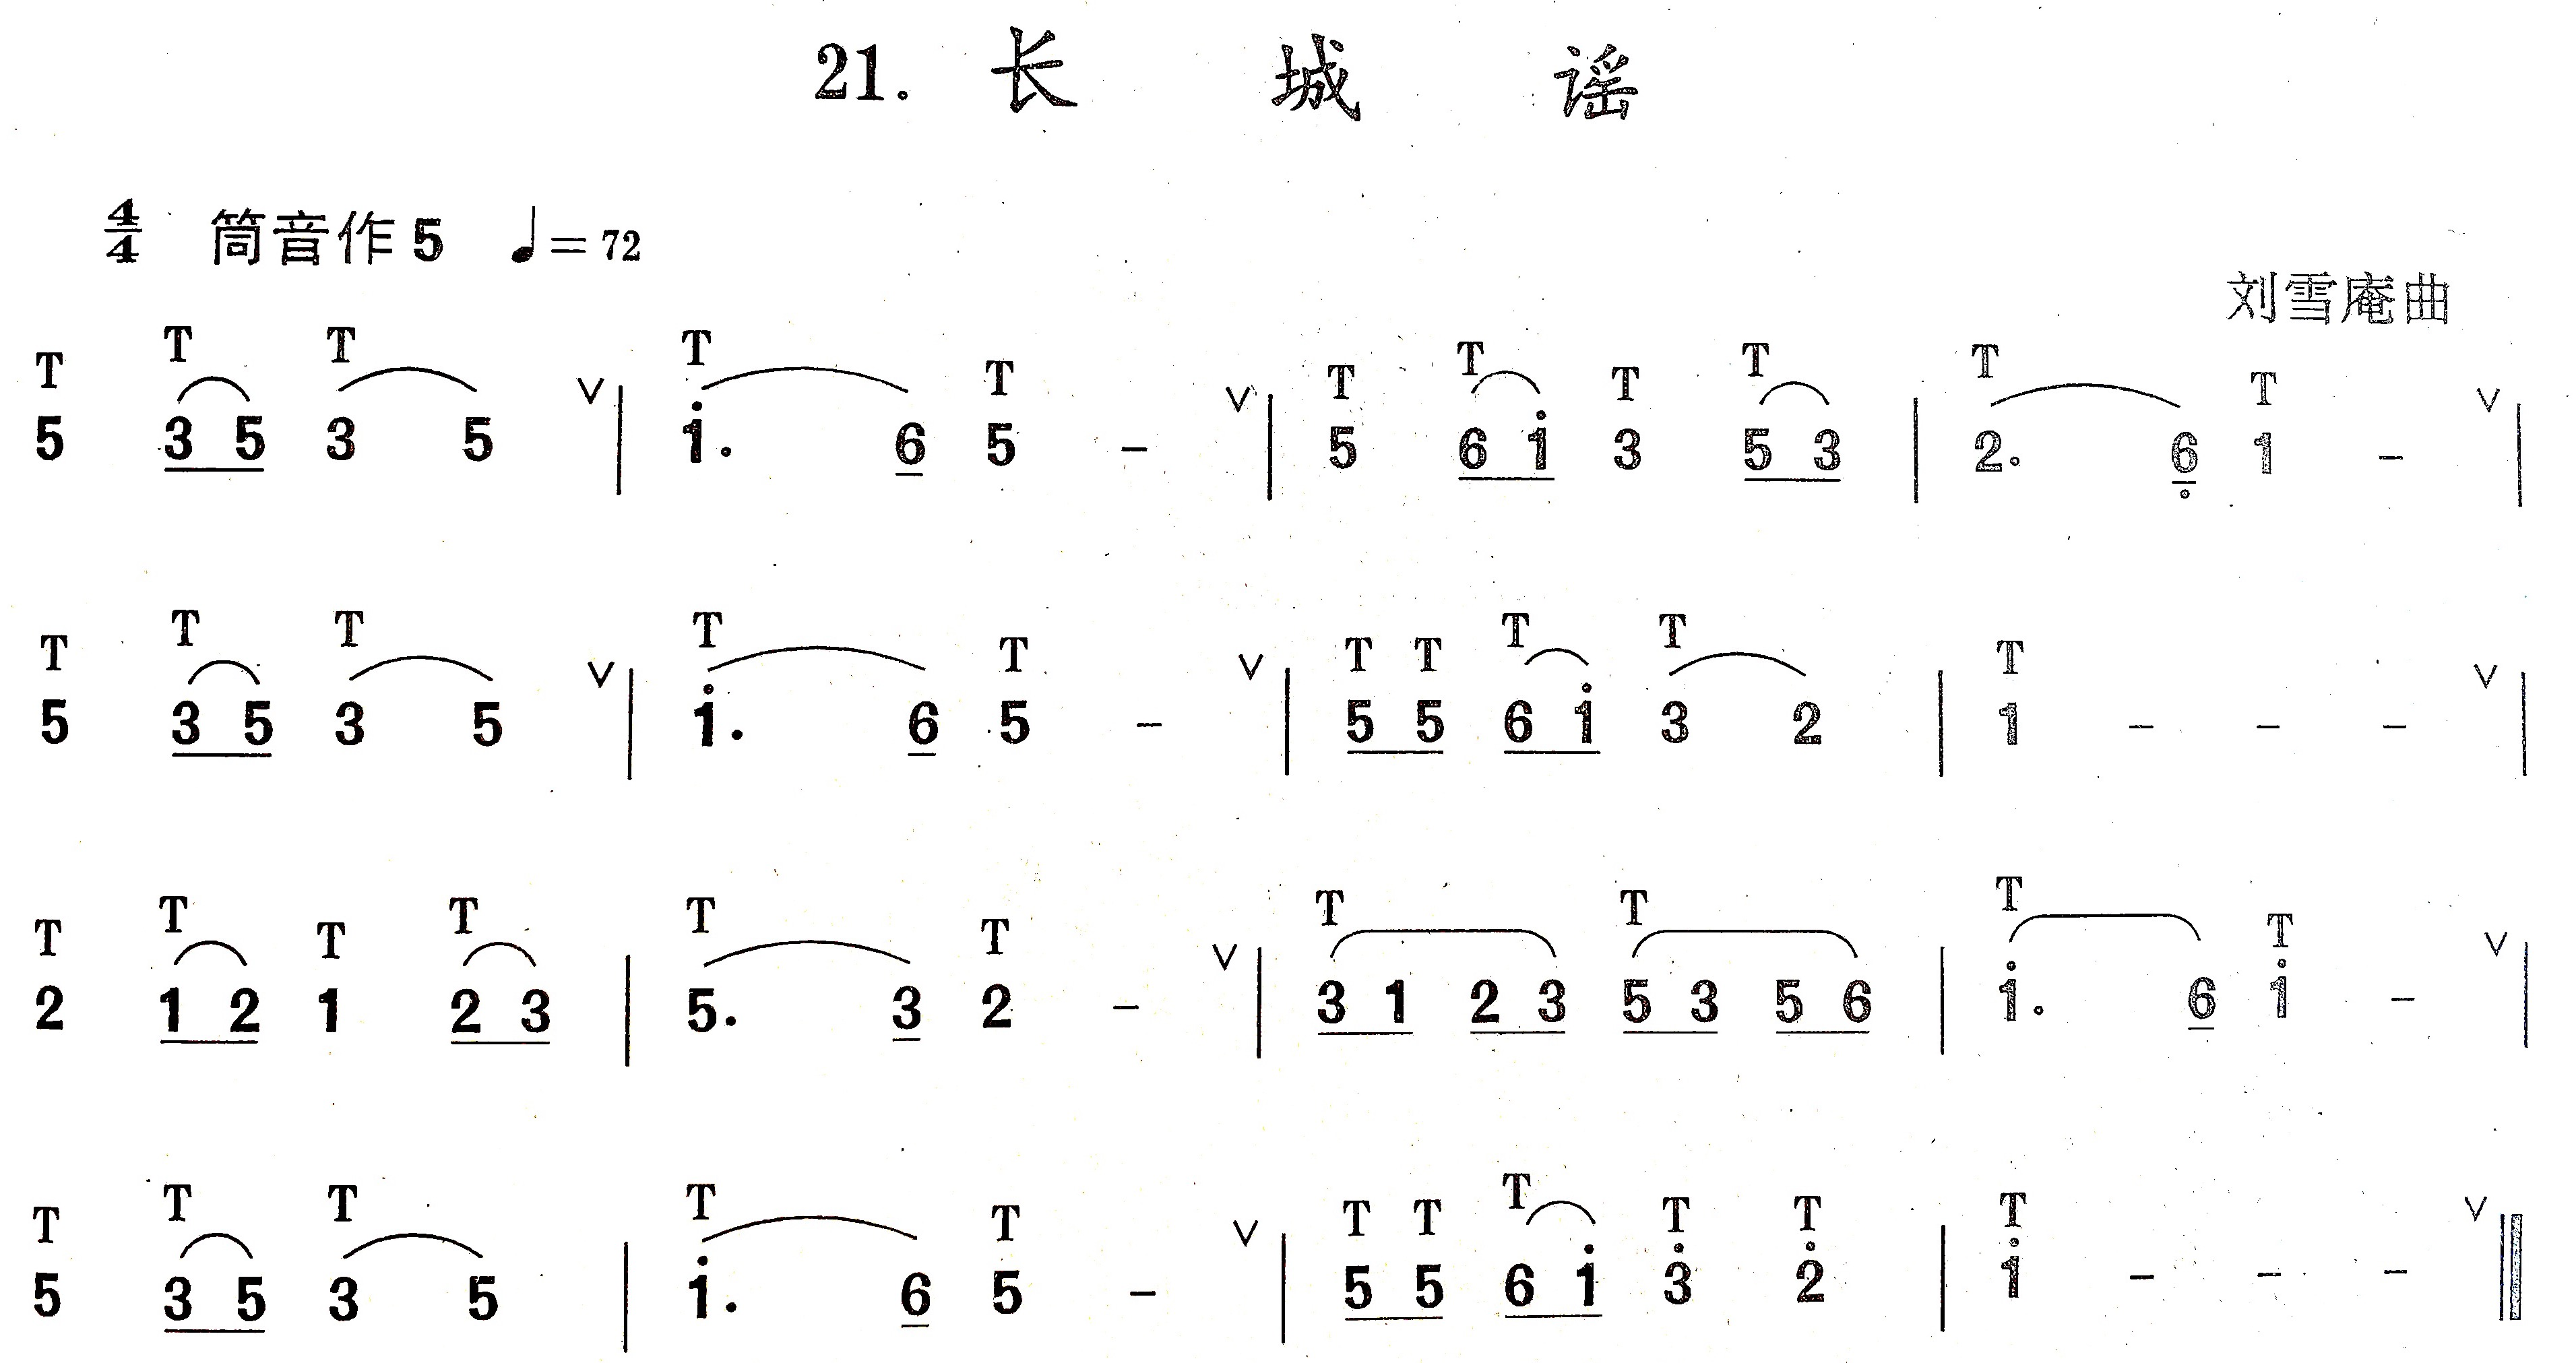
\includegraphics[width=\textwidth]{dongxiao/20200711-长城谣.jpg}
\section{西湖春}
    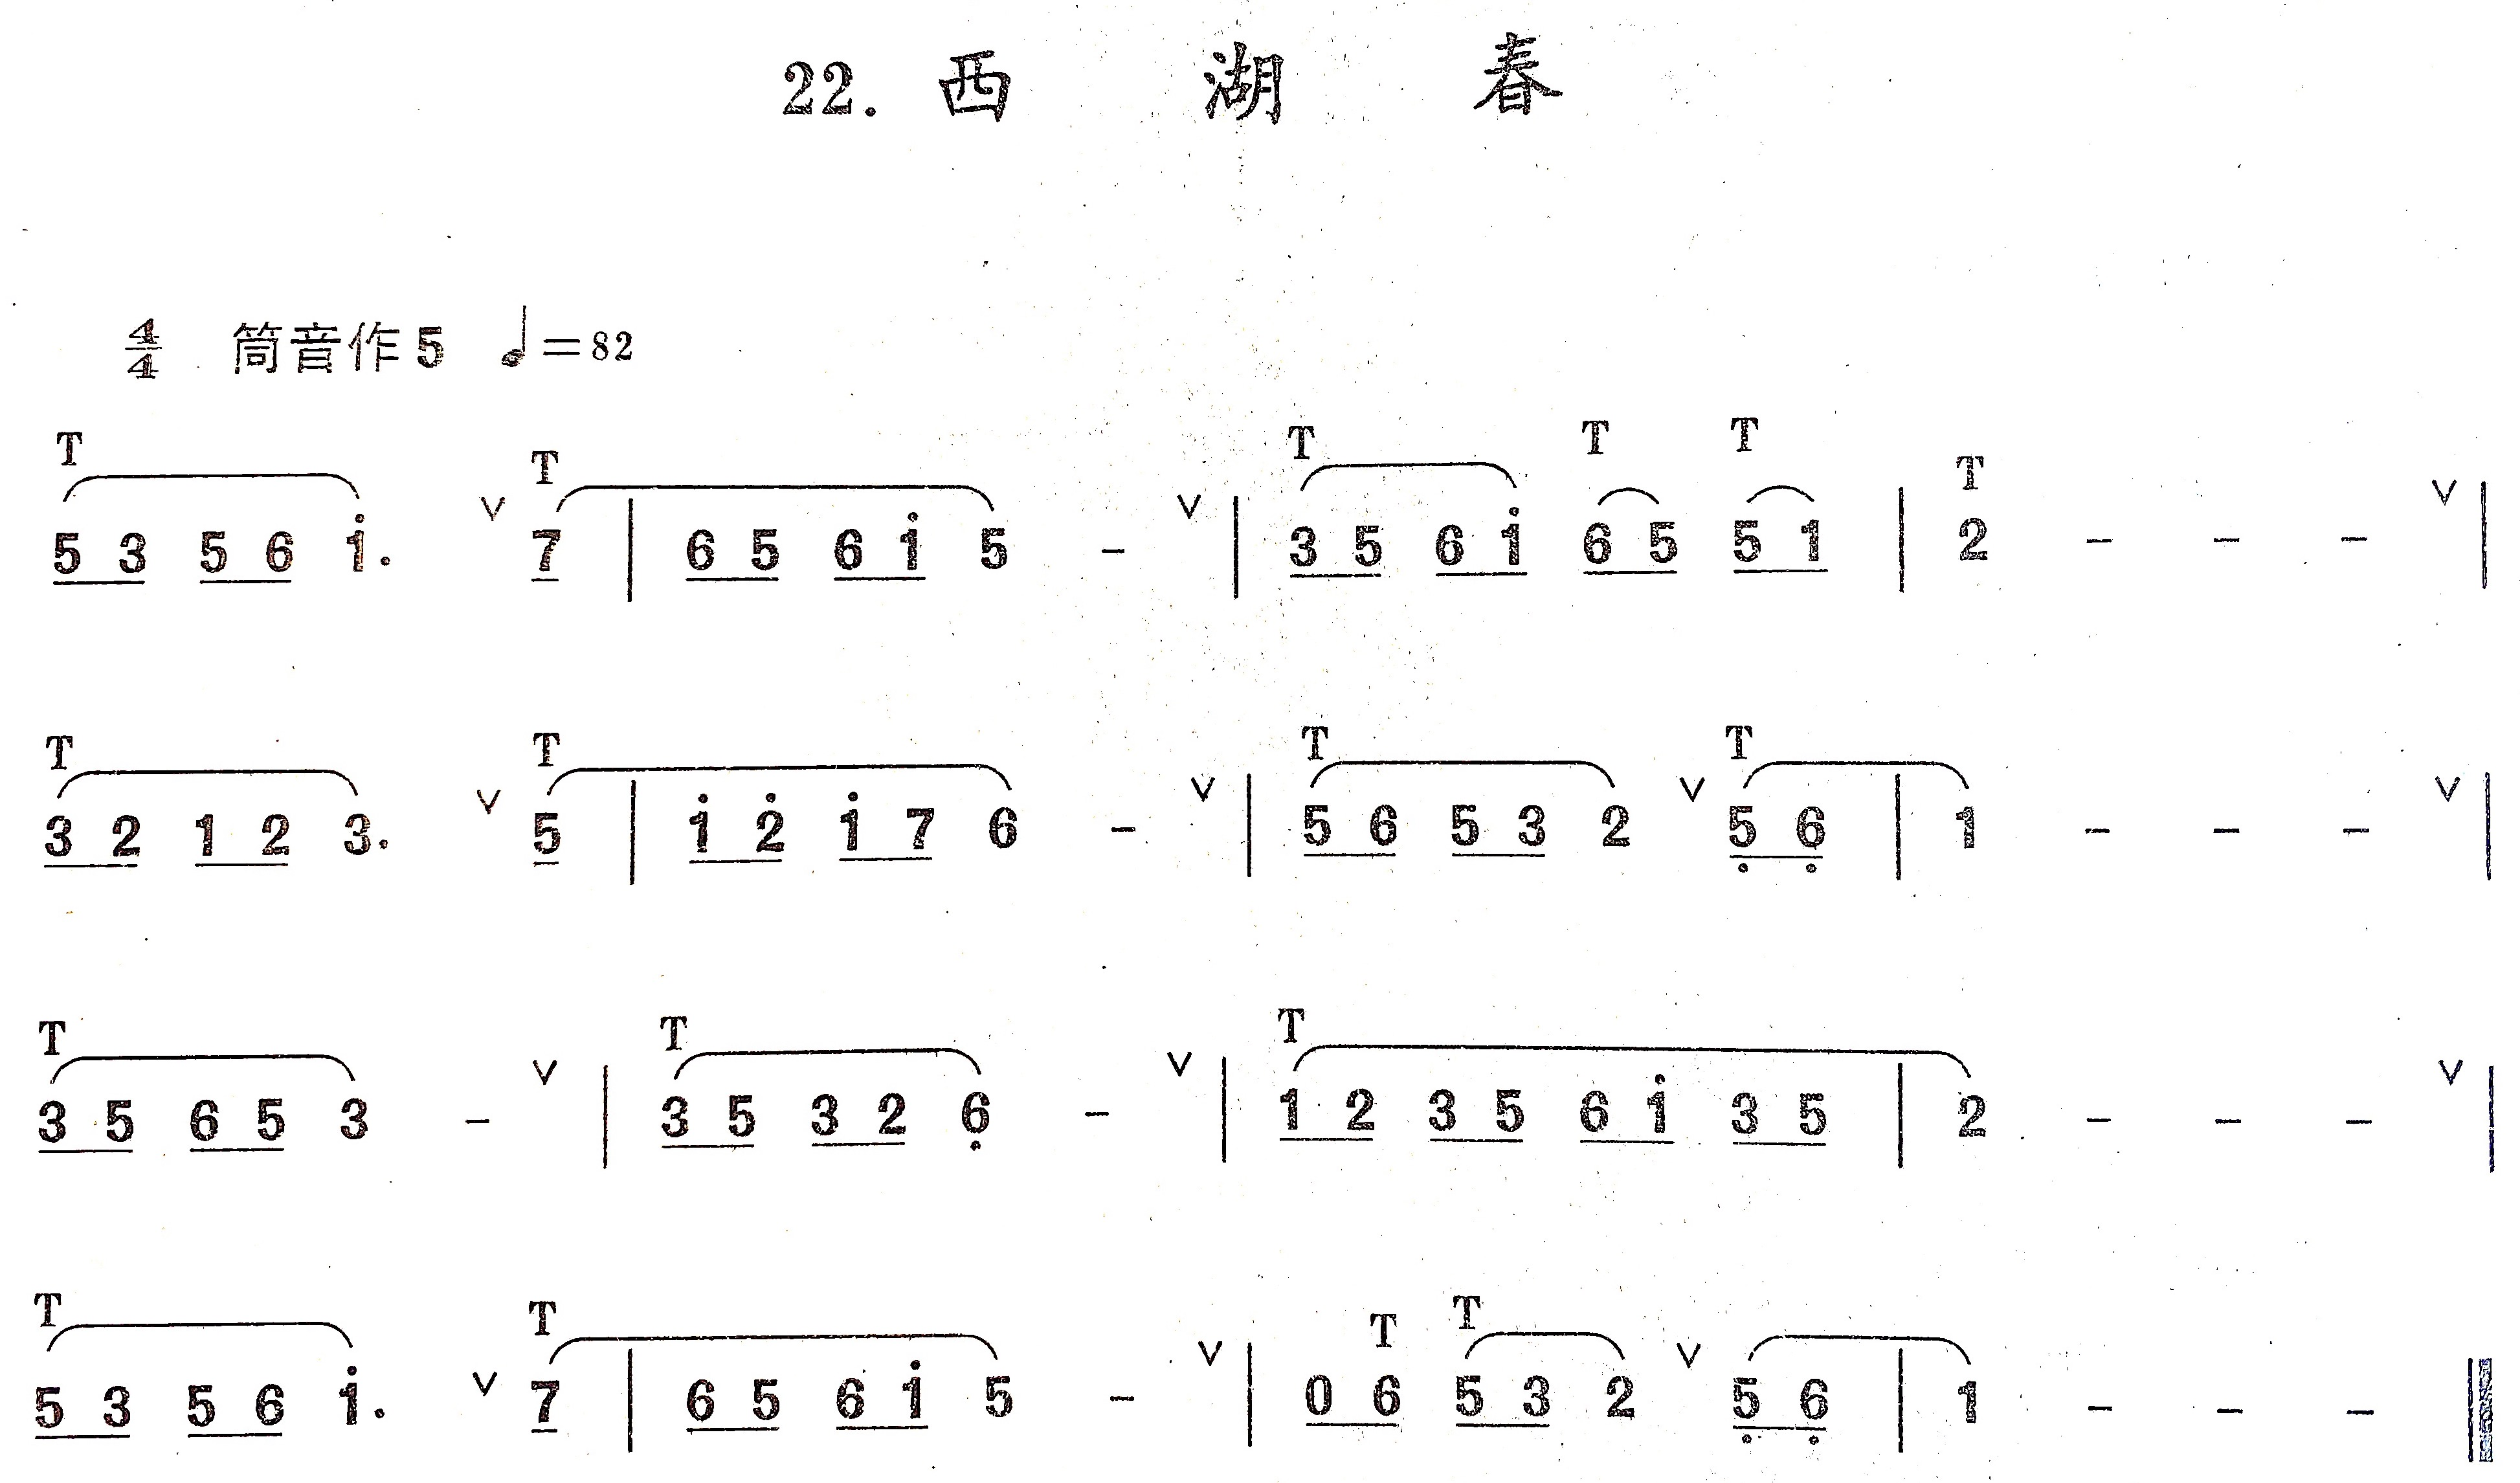
\includegraphics[width=\textwidth]{dongxiao/20200711-西湖春.jpg}
\section{茉莉花}
    \includegraphics[width=\textwidth]{dongxiao/20200711-茉莉花.jpg}

\section{無羈}
    \includegraphics[width=\textwidth]{dongxiao/20201231-無羈} 

\section{柳林坡}
    \includegraphics[width=\textwidth]{dongxiao/20201231-柳林坡}




\section{如花意梦}\includegraphics[width=\textwidth]{dongxiao/20200819/如花意梦.jpeg}
\section{愉快的梦}\includegraphics[width=\textwidth]{dongxiao/20200819/愉快的梦.jpeg}

\section{放风筝}\includegraphics[width=\textwidth]{dongxiao/20200819/放风筝.jpeg}

\section{明月清箫}\includegraphics[width=0.85\textwidth]{dongxiao/20200819/明月清箫.png}
\section{月牙五更}\includegraphics[width=\textwidth]{dongxiao/20200819/月牙五更.jpeg}
\section{木兰辞}\includegraphics[width=\textwidth]{dongxiao/20200819/木兰辞.jpeg}
\section{柳絮飞}\includegraphics[width=0.95\textwidth]{dongxiao/20200819/柳絮飞.jpg}

\chapter{牡丹亭}
\section{惊梦-山桃红}
    \includegraphics[width=0.95\textwidth]{mudanting/2021-牡丹亭-惊梦-山桃红.jpg}
\section{游园惊梦}
\paragraph*{\includegraphics[width=\textwidth]{mudanting/2020-牡丹亭-游园惊梦1}} 
\paragraph*{\includegraphics[width=0.95\textwidth]{mudanting/2020-牡丹亭-游园惊梦2}} \paragraph*{\includegraphics[width=0.95\textwidth]{mudanting/2020-牡丹亭-游园惊梦3}}
\paragraph*{\includegraphics[width=0.95\textwidth]{mudanting/2020-牡丹亭-游园惊梦4}}
\paragraph*{\includegraphics[width=0.95\textwidth]{mudanting/2020-牡丹亭-游园惊梦5}}
\paragraph*{\includegraphics[width=0.95\textwidth]{mudanting/2020-牡丹亭-游园惊梦6}}
\paragraph*{\includegraphics[width=\textwidth]{mudanting/2020-牡丹亭-游园惊梦7}}
           
\chapter{技巧練習}
\section{裝飾音}
    \includegraphics[width=0.9\textwidth]{dongxiao/20201231-裝飾音}
\section{氣震音}
    \includegraphics[width=0.8\textwidth]{dongxiao/Scan 8.jpeg}
\section{依音}
    \includegraphics[width=0.9\textwidth]{dongxiao/Scan 9.jpeg}
\section{波音}
    \includegraphics[width=0.9\textwidth]{dongxiao/Scan 10.jpeg}
\section{叠音}
    \includegraphics[width=0.9\textwidth]{dongxiao/Scan 11.jpeg}
\section{打音}
    \includegraphics[width=0.9\textwidth]{dongxiao/Scan 12.jpeg}
\section{厲音}
    \includegraphics[width=0.9\textwidth]{dongxiao/Scan 13.jpeg}
\section{滑音}
    \includegraphics[width=0.9\textwidth]{dongxiao/Scan 14.jpeg}
\section{吐音}
    \includegraphics[width=0.9\textwidth]{dongxiao/Scan 15.jpeg}

\newpage
\pagestyle{empty}
\includegraphics[width=\textwidth]{cover5}
\end{document}
